\documentclass[11pt]{article}

\usepackage[margin=1in]{geometry}
\usepackage[T1]{fontenc}
\usepackage{lmodern}
\usepackage{amsmath,amssymb,amsthm}
\usepackage{mathtools}
\numberwithin{equation}{section}
\usepackage{bm}
\usepackage{booktabs}
\usepackage{tabularx}
\usepackage{array}
\usepackage{graphicx}
\usepackage{siunitx}
\usepackage{xcolor}
\usepackage{enumitem}
\usepackage{microtype}
\usepackage{algorithm}
\usepackage{algpseudocode}
\usepackage{tikz}
\usetikzlibrary{arrows.meta,positioning,calc}
\usepackage[round,numbers,sort&compress]{natbib}
\usepackage[colorlinks=true,linkcolor=blue,citecolor=blue,urlcolor=blue]{hyperref}

% ---------------------------------------------------------------- shortcuts
\newcommand{\R}{\mathbb{R}}
\newcommand{\E}{\mathbb{E}}
\newcommand{\Prob}{\mathbb{P}}
\newcommand{\dd}{\,\mathrm{d}}
\newcommand{\pdd}[2]{\frac{\partial #1}{\partial #2}}
\newcommand{\pddt}[2]{\frac{\partial^{2} #1}{\partial #2^{2}}}
\newcommand{\norm}[1]{\left\lVert #1 \right\rVert}
\newcommand{\abs}[1]{\left\lvert #1 \right\rvert}
\newcommand{\xx}{\mathbf{x}}
\newcommand{\vv}{\mathbf{v}}
\newcommand{\ww}{\mathbf{w}}
\newcommand{\DD}{\mathbf{D}}
\newcommand{\nn}{\mathbf{n}}
\newcommand{\T}{\mathsf{T}}
\newcommand{\Pe}{\mathrm{Pe}}
\newcommand{\Da}{\mathrm{Da}}
\newcommand{\CVaR}{\operatorname{CVaR}}
\newcommand{\VaR}{\operatorname{VaR}}
\newcommand{\argmin}{\operatorname*{arg\,min}}
\newcommand{\argmax}{\operatorname*{arg\,max}}
\newcommand{\ind}{\mathbf{1}}
\newcommand{\ProbM}{\Prob_{M}}
\newcommand{\me}{\mathrm{e}}
\newcommand{\tabhead}[1]{\textbf{#1}}
\newcolumntype{Y}{>{\raggedright\arraybackslash}X}

\theoremstyle{plain}
\newtheorem{proposition}{Proposition}
\newtheorem{remark}{Remark}
\newtheorem{assumption}{Assumption}

\title{Stochastic Optimization of Pump-and-Treat Groundwater Remediation\\[2pt]
\large Random hydrological fields, fixed well layouts, and
chance-constrained pumping rates}
\author{Sergio Lucero}
\date{\today}

\begin{document}
\maketitle

\begin{abstract}
This document formulates and plans the solution of a stochastic
pump-and-treat remediation problem.  At least one hydrological field---first
and foremost the hydraulic conductivity---is modelled as a random field; the
optional random inputs include porosity, source strength and location,
boundary head, inlet concentration, and dispersivities.  The extraction wells
are placed at fixed, evenly distributed locations over a design plume; the
decision variables are the pumping rates.  The objective is the expected
life-cycle cost of pumping, treatment, and residual contamination.  The
constraints are well capacities, a total pumping budget, drawdown limits, and a
probabilistic compliance requirement at monitoring locations.  The result is a
PDE-constrained chance-constrained stochastic program.  We describe a
sample-average approximation (SAA), a conditional-value-at-risk (CVaR) and
smooth-sigmoid treatment of the chance constraint, adjoint and
surrogate-based gradient methods, and a gate-driven verification protocol.
The plan deliberately reuses the trusted one-, two-, and three-dimensional
forward models and the Fourier neural operator (FNO) work of the preceding
phases: the optimization layer is added only after the forward map has passed
its own accuracy gates.
\end{abstract}

\tableofcontents

% ======================================================================
\section{Scope and relation to the existing model chain}
\label{sec:scope}

The project already contains a verified forward chain:
\begin{enumerate}[leftmargin=1.6em,itemsep=2pt]
  \item a one-dimensional dimensionless advection--dispersion sandbox
        matching the Ogata--Banks solution to a relative $L^2$ error of
        $1.35\times10^{-2}$ on the full grid and $8.0\times10^{-3}$ in the
        interior \citep{ogata1961solution};
  \item two- and three-dimensional forward plans with Darcy flow, wells,
        random conductivity, finite-volume references, and
        physics-informed neural networks (PINNs)
        \citep{raissi2019pinn};
  \item a Fourier neural operator (FNO) program for learning the map from
        hydrological fields and well configurations to concentration fields
        \citep{li2021fno,kovachki2023neural}.
\end{enumerate}
The present document adds the \emph{decision} layer.  The logic is the same as
in the forward plans: add one new ingredient at a time, compare against a
reference that can be trusted, and do not advance until an explicit gate is
green.

\paragraph{The three objects of the optimization problem.}
\begin{enumerate}[leftmargin=1.6em,itemsep=2pt]
  \item \textbf{Uncertainty.}  A random field, primarily
        $K(\xx,\omega)$, plus optional random source and boundary data,
        described by a probability space $(\Theta,\mathcal{F},\Prob)$.
  \item \textbf{Decision.}  Extraction rates
        $\mathbf{q}(t)=(q_1(t),\dots,q_{N_w}(t))$ at fixed well locations
        $\xx_1,\dots,\xx_{N_w}$ that are evenly distributed over the design
        plume.  The locations are \emph{not} decision variables in the main
        problem; only the rates are.
  \item \textbf{Performance.}  Expected cost, reliability (probability of
        meeting the regulatory concentration), and robustness to distribution
        shift.
\end{enumerate}

\paragraph{What ``solve'' means here.}
The deliverable is not a single number.  A solution is
\begin{enumerate}[leftmargin=1.6em,itemsep=2pt]
  \item a well-defined stochastic program with existence and well-posedness
        assumptions;
  \item a tractable approximation (SAA, CVaR, smooth chance constraint);
  \item an algorithm with a verified gradient or a justified derivative-free
        alternative;
  \item an out-of-sample certificate: the optimized policy meets the
        reliability target on scenarios not used in optimization, and its
        cost is stable under a stated statistical error;
  \item a reproducible run manifest (config, seeds, scenario set, surrogate
        version, metrics).
\end{enumerate}

\paragraph{Notation.}
Table~\ref{tab:notation} fixes the symbols.  The subscript $i$ always refers
to a well, $m$ to a Monte Carlo scenario, and $c$ to a compliance location.
The superscript $(0)$ denotes a background (no-pumping) quantity and $(i)$ a
unit-rate response of well $i$.

\begin{table}[htbp]
\centering
\small
\begin{tabularx}{\textwidth}{@{}lY@{}}
\toprule
\tabhead{Symbol} & \tabhead{Meaning}\\
\midrule
$\Omega\subset\R^d$, $d\in\{2,3\}$ & Aquifer domain; $d=2$ is depth-averaged,
$d=3$ is full three-dimensional\\
$\partial\Omega=\Gamma_D\cup\Gamma_N\cup\Gamma_{\mathrm{in}}\cup
 \Gamma_{\mathrm{out}}$ & Dirichlet, no-flow, inflow, and outflow boundaries\\
$\xx$, $t$, $T$ & Space, time, and remediation horizon\\
$(\Theta,\mathcal{F},\Prob)$ & Probability space; $\omega\in\Theta$ is a
scenario\\
$K(\xx,\omega)$, $K_0$, $G$ & Hydraulic conductivity, geometric mean, and
$\log K$\\
$\phi(\xx,\omega)$, $R$ & Porosity and retardation factor\\
$h(\xx,t,\omega)$ & Hydraulic head\\
$\ww=-K\nabla h$, $\vv=\ww/\phi$ & Darcy flux and seepage (pore) velocity\\
$C(\xx,t,\omega)$ & Dissolved concentration\\
$C_0$, $C_{\mathrm{reg}}$ & Reference and regulatory concentrations\\
$q_i(t)$, $\mathbf{q}(t)$ & Extraction rate of well $i$ and rate vector\\
$\xx_i$, $N_w$ & Fixed well location and number of wells\\
$Q_{\max}$, $q_i^{\max}$ & Plant capacity and per-well capacity\\
$h_{\min}(\xx)$ & Minimum allowable head (drawdown constraint)\\
$\DD$, $\alpha_L$, $\alpha_T$ & Dispersion tensor and longitudinal/transverse
dispersivities\\
$\lambda$, $S_b$ & First-order decay rate and background source\\
$\mathcal{M}_c$ & Set of compliance monitoring locations\\
$\mathcal{O}_h$ & Set of head observation locations\\
$\tau_c(\mathbf{q},\omega)$ & Cleanup time to reach $C_{\mathrm{reg}}$\\
$J(\mathbf{q},\omega)$ & Cost of one scenario\\
$G(\mathbf{q},\omega)$, $H(\mathbf{q},\omega)$ & Compliance and drawdown
violation functions\\
$\alpha$, $\alpha_h$ & Allowed compliance and drawdown violation
probabilities\\
$M$ & Number of SAA scenarios\\
$c_e,c_w,c_m,c_\tau$ & Pumping, treatment, residual-mass, and cleanup-time
cost coefficients\\
\bottomrule
\end{tabularx}
\caption{Notation used throughout the optimization formulation.}
\label{tab:notation}
\end{table}

% ======================================================================
\section{Deterministic forward model for a fixed scenario}
\label{sec:forward}

For a fixed realization $\omega$ and a fixed rate vector $\mathbf{q}$, the
state is the pair $(\mathbf{h},\mathbf{C})$.  The flow and transport equations
are deliberately kept in the same form as in the forward plans; the only new
terms are the extraction wells and the explicit dependence on $\mathbf{q}$.

\subsection{Flow with extraction wells}
\label{sec:flow}

For a confined, constant-density aquifer,
\begin{equation}
\label{eq:flow}
S_s\pdd{h}{t}
-\nabla\cdot(K\nabla h)
= W_b(\xx,t,\omega)
-\sum_{i=1}^{N_w} q_i(t)\,\delta_{\varepsilon}(\xx-\xx_i),
\qquad (\xx,t)\in\Omega\times(0,T],
\end{equation}
with
\begin{equation}
\label{eq:darcy}
\ww=-K\nabla h,
\qquad
\vv=\frac{\ww}{\phi}.
\end{equation}
Here $W_b$ is a background source/recharge (injection positive), $q_i(t)\ge0$
is the extraction rate of well $i$, and $\delta_{\varepsilon}$ is a
regularized delta function of width $\varepsilon$ (Section~\ref{sec:wellreg}).
For steady flow, the storage term is dropped and \eqref{eq:flow} becomes an
elliptic equation.  The boundary and initial conditions are
\begin{equation}
\label{eq:flowbc}
h=h_D\ \text{on }\Gamma_D,
\qquad
-K\nabla h\cdot\nn=g_N\ \text{on }\Gamma_N,
\qquad
h(\xx,0)=h_0(\xx).
\end{equation}
For an anisotropic aquifer, $K$ in \eqref{eq:flow} is the symmetric positive
definite tensor $\operatorname{diag}(K_h,K_h,K_v)$ in three dimensions; the
two-dimensional model uses the transmissivity $T=Kb$, with $b$ the aquifer
thickness.

\paragraph{Linear superposition in the pumping rates.}
For fixed $K$ and fixed boundary data, \eqref{eq:flow} is linear in
$\mathbf{q}$.  Its solution can be written as
\begin{equation}
\label{eq:superposition}
h(\xx,t;\mathbf{q},\omega)
=h^{(0)}(\xx,t,\omega)
+\sum_{i=1}^{N_w} q_i(t)\,h^{(i)}(\xx,t,\omega),
\end{equation}
where $h^{(0)}$ is the no-pumping head and $h^{(i)}$ is the head generated by
a unit extraction rate at well $i$.  Consequently
\begin{equation}
\label{eq:vsuper}
\vv(\xx,t;\mathbf{q},\omega)
=\vv^{(0)}(\xx,t,\omega)
+\sum_{i=1}^{N_w} q_i(t)\,\vv^{(i)}(\xx,t,\omega).
\end{equation}
This superposition is the main computational advantage of the flow model: for
each scenario one solves $N_w+1$ linear flow problems, after which the
velocity field for \emph{any} rate vector is a linear combination.  It also
gives the derivative $\partial\vv/\partial q_i=\vv^{(i)}$ used in the adjoint
and in the surrogate parameterization.

\subsection{Transport with extraction wells}
\label{sec:transport}

The conservative advection--dispersion equation with linear equilibrium
sorption and first-order decay is
\begin{equation}
\label{eq:transport}
R\phi\pdd{C}{t}
+\nabla\cdot(\phi\vv C)
-\nabla\cdot(\phi\DD\nabla C)
+\lambda R\phi C
=S_b(\xx,t,\omega),
\end{equation}
where $R=1+\rho_bK_d/\phi$ and $\lambda\ge0$.  The velocity $\vv$ in
\eqref{eq:transport} is the \emph{full} velocity \eqref{eq:vsuper}, including
the pumping.  The extraction wells therefore do not need a separate sink term:
in the non-conservative form,
\begin{equation}
\label{eq:divv}
\nabla\cdot(\phi\vv C)
=\phi\vv\cdot\nabla C
+C\,\nabla\cdot(\phi\vv),
\qquad
\nabla\cdot(\phi\vv)
=W_b-\sum_{i=1}^{N_w}q_i\delta_{\varepsilon}(\xx-\xx_i),
\end{equation}
so the term $-C\sum_i q_i\delta_{\varepsilon}$ removes mass at the wells.  In
a finite-volume discretization the well cells are sink cells and the upwind
advective flux removes mass consistently.  If a non-conservative form
$\phi\vv\cdot\nabla C$ is used instead, the explicit sink
$-\sum_i q_i C\delta_{\varepsilon}$ must be added; forgetting it is a common
and silent mass-balance error.

The dispersion tensor is
\begin{equation}
\label{eq:D2}
\DD=\alpha_T\abs{\vv}\mathbf{I}
+(\alpha_L-\alpha_T)\frac{\vv\vv^{\T}}{\abs{\vv}}
+D_m\tau_m\mathbf{I},
\end{equation}
with molecular diffusion $D_m$ and tortuosity $\tau_m$; in most runs the
molecular term is absorbed into $\alpha_T$.  In three dimensions,
$\alpha_T$ is replaced by a horizontal transverse dispersivity
$\alpha_{TH}$ and a vertical transverse dispersivity $\alpha_{TV}$.  The
longitudinal and transverse dispersion coefficients are
$D_L=\alpha_L\abs{\vv}$ and $D_T=\alpha_T\abs{\vv}$; their ratio
$r=D_L/D_T=\alpha_L/\alpha_T$ controls plume elongation.

The boundary and initial conditions are
\begin{equation}
\label{eq:transportbc}
\begin{aligned}
C&=C_{\mathrm{in}}(\xx,t,\omega)
&&\text{on }\Gamma_{\mathrm{in}},\\
\DD\nabla C\cdot\nn&=0
&&\text{on }\Gamma_{\mathrm{out}}\cup\Gamma_N,\\
C(\xx,0)&=C_0(\xx,\omega)&&\text{in }\Omega.
\end{aligned}
\end{equation}
On \eqref{eq:transportbc}, $\vv\cdot\nn=0$ on $\Gamma_N$, so
$\DD\nabla C\cdot\nn=0$ is the no-flux condition there; on
$\Gamma_{\mathrm{out}}$ the same condition is the standard zero-diffusive
flux condition, which allows advective outflow.  A far-field Dirichlet
condition $C=0$ is also acceptable if the domain is large enough that the
plume never reaches the boundary.  The choice must be recorded in the run
manifest because it changes the extracted-mass accounting.

\paragraph{Mass balance.}
For \eqref{eq:transport} with the outflow condition,
\begin{equation}
\label{eq:massbalance}
\frac{\dd}{\dd t}\int_\Omega R\phi C\dd\xx
=\int_\Omega S_b\dd\xx
-\int_{\Gamma_{\mathrm{out}}}\phi\vv\cdot\nn\,C\dd A
-\int_\Omega\lambda R\phi C\dd\xx
-\sum_{i=1}^{N_w}q_iC(\xx_i,t).
\end{equation}
The last term is the mass removed by the wells.  Equation~\eqref{eq:massbalance}
is the primary diagnostic for the transport solver and for the surrogate: a
policy that looks cheap because it violates mass balance is not a solution.

\subsection{Well regularization and screened wells}
\label{sec:wellreg}

A point well gives a logarithmic singularity in $h$ and a $1/r$ singularity in
$\vv$.  The singularity is physical near the well but is not resolvable on a
coarse grid, and it contaminates error metrics.  We therefore replace the
delta function by a radial kernel
\begin{equation}
\label{eq:deltaeps}
\delta_{\varepsilon}(\xx-\xx_i)
=\frac{1}{(2\pi\varepsilon^2)^{d/2}}
\exp\!\left(-\frac{\abs{\xx-\xx_i}^2}{2\varepsilon^2}\right),
\end{equation}
with $\varepsilon$ of the order of one or two grid cells and no smaller than
the well radius $r_w$.  For a well screened over the interval
$[z_i^b,z_i^t]$ in three dimensions,
\begin{equation}
\label{eq:screened}
\delta_{\varepsilon,s}(\xx-\xx_i)
=\frac{1}{\ell_{s,i}}\ind_{[z_i^b,z_i^t]}(z)\,
\delta_{\varepsilon}(\xx_h-\xx_{h,i}),
\qquad
\ell_{s,i}=z_i^t-z_i^b,
\end{equation}
where $\xx_h$ is the horizontal coordinate.  This distributes the rate over
the screened cells and avoids a point source at the screen.

\begin{remark}[Units]
In three dimensions $q_i$ has units $\si{L^3.T^{-1}}$; in a depth-averaged
two-dimensional model it has units $\si{L^2.T^{-1}}$ (volume per unit
thickness per time).  The cost coefficients in Section~\ref{sec:cost} carry
the corresponding units.  The implementation uses a single
\texttt{dimension} flag and converts at the boundary of the optimization
layer.
\end{remark}

\subsection{Dimensionless form and groups}
\label{sec:nondim}

The forward plans use dimensionless variables because they keep residuals and
loss terms $\mathcal{O}(1)$.  The optimization layer inherits the same scales.
Let $L$ be a length scale, $H_0$ a head scale, $K_0$ the geometric mean
conductivity, $\phi_0$ a reference porosity, $U=K_0H_0/(\phi_0L)$ a reference
pore velocity, $T_0=L/U$, $C_0$ a reference concentration, and
\begin{equation}
\label{eq:Q0}
Q_0=\phi_0UL^{d-1}
\end{equation}
a reference pumping rate.  Define
\begin{equation}
\label{eq:nondimvars}
\xi=\frac{\xx}{L},\quad
\tau=\frac{t}{T_0},\quad
\tilde h=\frac{h}{H_0},\quad
\tilde C=\frac{C}{C_0},\quad
\tilde K=\frac{K}{K_0},\quad
\tilde\phi=\frac{\phi}{\phi_0},\quad
\tilde q_i=\frac{q_i}{Q_0}.
\end{equation}
The flow equation becomes
\begin{equation}
\label{eq:flownd}
-\nabla_{\xi}\cdot(\tilde K\nabla_{\xi}\tilde h)
=\tilde W_b-\sum_{i=1}^{N_w}\tilde q_i\,\tilde\delta_{\varepsilon},
\end{equation}
and the transport equation becomes
\begin{equation}
\label{eq:transportnd}
R\tilde\phi\,\tilde C_{\tau}
+\nabla_{\xi}\cdot(\tilde\phi\tilde{\vv}\tilde C)
-\frac{1}{\Pe_L}\nabla_{\xi}\cdot
 \bigl(\tilde\phi\tilde{\DD}\nabla_{\xi}\tilde C\bigr)
+\Da R\tilde\phi\tilde C
=\tilde S_b,
\end{equation}
with
\begin{equation}
\label{eq:groups}
\Pe_L=\frac{UL}{D_{L0}},\qquad
\tilde{\DD}=\frac{\DD}{D_{L0}},\qquad
\Da=\lambda T_0,\qquad
\tilde W_b=\frac{W_bL^2}{K_0H_0},\qquad
\tilde\delta_{\varepsilon}=L^d\delta_{\varepsilon},\qquad
\tilde S_b=\frac{S_bT_0}{\phi_0RC_0},
\end{equation}
where $D_{L0}=\alpha_LU$ is a reference longitudinal dispersion.  In the
isotropic case $\tilde{\DD}=\mathbf{I}$ and \eqref{eq:transportnd} reduces to
the trusted dimensionless ADE.  The transverse-to-longitudinal ratio is
$r=D_L/D_T=\alpha_L/\alpha_T$; in three dimensions the vertical anisotropy is
$\kappa=K_v/K_h$ and the aspect ratio is $\epsilon=H/L$.

The decision-relevant dimensionless groups are collected in
Table~\ref{tab:groups}.  A run manifest must report all of them, together with
the random-field parameters $(\sigma_G,\ell)$ and the well count $N_w$.

\begin{table}[htbp]
\centering
\small
\begin{tabularx}{\textwidth}{@{}lY@{}}
\toprule
\tabhead{Group} & \tabhead{Interpretation / role in optimization}\\
\midrule
$\Pe_L=UL/D_{L0}$ & Advection versus longitudinal dispersion; controls front
sharpness and the value of pumping\\
$r=D_L/D_T=\alpha_L/\alpha_T$ & Plume elongation; controls whether transverse
wells are useful\\
$\Da=\lambda T_0$ & Decay over the remediation horizon; reduces the required
pumping\\
$R$ & Retardation; delays breakthrough and cleanup\\
$\kappa=K_v/K_h$ & Vertical anisotropy; controls vertical well capture in 3D\\
$\tilde q_i=q_i/Q_0$ & Dimensionless extraction rate; decision variable\\
$\tilde C_{\mathrm{reg}}=C_{\mathrm{reg}}/C_0$ & Regulatory threshold in
dimensionless form\\
$\tilde h_{\min}=h_{\min}/H_0$ & Drawdown limit in dimensionless form\\
$\sigma_G$, $\ell/L$ & Log-conductivity standard deviation and correlation
length; control uncertainty and scenario dimension\\
$M$, $\alpha$ & SAA sample size and allowed compliance violation\\
\bottomrule
\end{tabularx}
\caption{Dimensionless groups and parameters that must accompany every
stochastic optimization run.}
\label{tab:groups}
\end{table}

\paragraph{Cost scaling.}
Costs are dimensional, but the optimizer benefits from an $\mathcal{O}(1)$
objective.  Let
\begin{equation}
\label{eq:J0}
J_0=c_eQ_0T_0N_w
\end{equation}
be a reference pumping cost.  The dimensionless coefficients are
\begin{equation}
\label{eq:cscaled}
\tilde c_e=1,\qquad
\tilde c_w=\frac{c_wC_0Q_0T_0}{J_0},\qquad
\tilde c_m=\frac{c_m\phi_0RC_0\abs{\Omega}}{J_0},\qquad
\tilde c_\tau=\frac{c_\tau T_0}{J_0}.
\end{equation}
The optimizer works with $\tilde c_\bullet$ and reports the dimensional cost
by multiplying back by $J_0$.

\subsection{Well-posedness assumptions}
\label{sec:wellposed}

The following assumptions are sufficient for the forward map and for the
optimization formulation.  They are stated explicitly because the chance
constraint and the adjoint require differentiability and uniform ellipticity.

\begin{assumption}[Ellipticity and boundedness]
\label{ass:elliptic}
There exist constants $0<K_{\min}\le K_{\max}<\infty$ such that
$K_{\min}\le K(\xx,\omega)\le K_{\max}$ for almost every
$(\xx,\omega)\in\Omega\times\Theta$.  The porosity satisfies
$0<\phi_{\min}\le\phi\le\phi_{\max}<\infty$.  The log-conductivity is a
truncated Gaussian field with a continuous, positive-definite covariance.
\end{assumption}

\begin{assumption}[Regularity]
\label{ass:regularity}
The domain $\Omega$ is bounded with a Lipschitz boundary.  The boundary data
$h_D$, $g_N$, $C_{\mathrm{in}}$, and the source $S_b$ are sufficiently smooth
that the flow and transport problems have unique weak solutions for every
$\omega$ and every admissible $\mathbf{q}$.
\end{assumption}

\begin{assumption}[Well regularization]
\label{ass:wellreg}
The regularized wells satisfy $\delta_{\varepsilon}\in L^\infty(\Omega)$,
$\delta_{\varepsilon}\ge0$, $\int_\Omega\delta_{\varepsilon}\dd\xx=1$, and
$\operatorname{supp}\delta_{\varepsilon}(\cdot-\xx_i)\subset\Omega$ for every
$i$.  The regularization width $\varepsilon$ is fixed before optimization and
is not a decision variable.
\end{assumption}

Under these assumptions, the flow problem is uniformly elliptic and the
transport problem is a uniformly parabolic advection--diffusion--reaction
equation with bounded coefficients.  The state map
$\mathcal{S}:(\mathbf{q},\omega)\mapsto(\mathbf{h},\mathbf{C})$ is well
defined.  The only non-smoothness in the forward map comes from the
maxima/minima in the compliance and drawdown functions and from the
indicator in the empirical chance constraint; both are handled explicitly in
Section~\ref{sec:saa}.

% ======================================================================
\section{Well layout: evenly distributed wells in the plume}
\label{sec:wells}

\subsection{Design plume and here-and-now locations}

The wells are placed before the uncertainty is realized.  Their locations
therefore cannot depend on $\omega$.  We define a \emph{design plume}
$\Omega_p\subset\Omega$ from a reference scenario or from a probability
contour,
\begin{equation}
\label{eq:designplume}
\Omega_p
=\left\{\xx\in\Omega:\ \E\bigl[C_{\mathrm{ref}}(\xx,T_d)\bigr]\ge c_p\right\}
\quad\text{or}\quad
\Omega_p
=\left\{\xx\in\Omega:\ \Prob\bigl(C_{\mathrm{ref}}(\xx,T_d)\ge c_p\bigr)
\ge1-\beta\right\},
\end{equation}
where $C_{\mathrm{ref}}$ is the concentration under a reference policy (for
example, no pumping or a nominal pumping rate), $T_d$ is a design time, and
$c_p$ is a plume threshold.  The second form is more conservative and is
preferred when the plume footprint is highly uncertain.  The design plume
should cover the union of the likely footprints, not only the mean plume; a
well that is outside the plume in every scenario is wasted, but a well that is
outside the plume in the mean and inside it in the upper tail can be valuable.

\subsection{Hexagonal lattice}

For a compact, roughly convex design plume, the default layout is a hexagonal
(triangular) lattice.  If $A_p=\abs{\Omega_p}$ is the plume area and $N_w$ the
number of wells, the lattice spacing is
\begin{equation}
\label{eq:hexspacing}
\ell_w=\sqrt{\frac{2A_p}{\sqrt{3}\,N_w}}.
\end{equation}
The candidate locations are
\begin{equation}
\label{eq:hexpoints}
\xx_{i_1i_2}
=\xx_c+\ell_w\left(i_1+\frac{i_2}{2},\ \frac{\sqrt{3}}{2}i_2\right),
\qquad (i_1,i_2)\in\mathbb{Z}^2,
\end{equation}
where $\xx_c$ is the plume centroid.  Retain the $N_w$ points that lie in
$\Omega_p$ and are closest to $\xx_c$; if the count is not exact, adjust the
spacing by a one-dimensional root find or add/remove boundary points.  The
hexagonal lattice minimizes the covering radius for a given number of points
and gives a natural $60^\circ$ spacing between neighboring wells.  The
covering radius is approximately $\ell_w/\sqrt{3}$; it is a useful diagnostic
for whether the well spacing is compatible with the expected capture-zone
radius.

\subsection{Centroidal Voronoi tessellation for irregular plumes}

For an irregular plume, a hexagonal lattice clipped to $\Omega_p$ leaves
uneven gaps.  A better general construction is a centroidal Voronoi
tessellation (CVT).  Given $N_w$ points $\xx_i$, define the Voronoi cells
\begin{equation}
\label{eq:voronoi}
V_i=\left\{\xx\in\Omega_p:\ \abs{\xx-\xx_i}\le\abs{\xx-\xx_j}
\ \forall j\ne i\right\}.
\end{equation}
The CVT minimizes the quantization error
\begin{equation}
\label{eq:cvt}
\min_{\xx_1,\dots,\xx_{N_w}}
\sum_{i=1}^{N_w}\int_{V_i}\abs{\xx-\xx_i}^2\dd\xx,
\end{equation}
and is computed by Lloyd's algorithm: initialize with a low-discrepancy point
set in $\Omega_p$, compute the Voronoi cells, move each point to the centroid
of its cell, and repeat until the points move less than a tolerance.  The
result is an evenly distributed set of wells that adapts to the plume shape.
The CVT is the default for non-convex or highly irregular design plumes; the
hexagonal lattice is the default for compact plumes because it is
reproducible and has a closed-form spacing.

\begin{figure}[htbp]
\centering
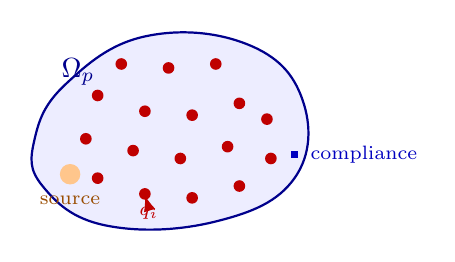
\begin{tikzpicture}[scale=1.0]
  % design plume
  \fill[blue!7]
    plot[smooth cycle,tension=0.7]
    coordinates {(0.2,0.7) (1.0,0.2) (2.4,0.25) (3.4,0.8)
                 (3.5,1.8) (2.8,2.5) (1.5,2.6) (0.5,2.0) (0.1,1.3)};
  \draw[thick,blue!55!black]
    plot[smooth cycle,tension=0.7]
    coordinates {(0.2,0.7) (1.0,0.2) (2.4,0.25) (3.4,0.8)
                 (3.5,1.8) (2.8,2.5) (1.5,2.6) (0.5,2.0) (0.1,1.3)};
  \node[blue!55!black] at (0.65,2.15) {$\Omega_p$};
  % source zone
  \fill[orange!45] (0.55,0.85) circle (0.13);
  \node[font=\scriptsize,orange!60!black] at (0.55,0.52) {source};
  % wells
  \foreach \x/\y in {
    0.9/0.8, 1.5/0.6, 2.1/0.55, 2.7/0.7, 3.1/1.05,
    0.75/1.3, 1.35/1.15, 1.95/1.05, 2.55/1.2, 3.05/1.55,
    0.9/1.85, 1.5/1.65, 2.1/1.6, 2.7/1.75,
    1.2/2.25, 1.8/2.2, 2.4/2.25}
    \fill[red!75!black] (\x,\y) circle (2.1pt);
  \node[red!75!black,font=\scriptsize] at (1.55,0.35) {$q_i$};
  \draw[-{Latex[length=2mm]},red!75!black] (1.55,0.42) -- (1.5,0.58);
  % compliance well
  \fill[blue!75!black] (3.35,1.05) rectangle ++(0.1,0.1);
  \node[blue!75!black,font=\scriptsize,right] at (3.48,1.10)
    {compliance};
\end{tikzpicture}
\caption{Schematic of the fixed well layout.  The design plume $\Omega_p$ is
the region used to place the $N_w$ extraction wells; the red dots are the
fixed locations $\xx_i$, and the decision variables are the rates $q_i\ge0$.
The blue square is a compliance monitoring location.  The layout is
here-and-now: it does not change with the random realization $\omega$.}
\label{fig:wells}
\end{figure}

\paragraph{What is \emph{not} optimized.}
The main problem treats $\xx_i$ as fixed.  Optimizing the locations as well is
a separate mixed-integer design problem: it introduces binary variables, a
combinatorial number of layouts, and a different set of well-spacing
constraints.  Section~\ref{sec:placement} sketches that extension.  The
present document keeps the locations fixed so that the stochastic program is
continuous in the decision variables and the adjoint/surrogate machinery can
be verified cleanly.

% ======================================================================
\section{Stochastic model}
\label{sec:stochastic}

\subsection{Probability space and random inputs}

Let $(\Theta,\mathcal{F},\Prob)$ be a complete probability space.  The primary
random field is the hydraulic conductivity, but the formulation is written for
a vector of random inputs so that additional fields can be switched on
without changing the optimization algorithm.  Table~\ref{tab:random} lists
the supported inputs, their default distributions, and their role.

\begin{table}[htbp]
\centering
\small
\begin{tabularx}{\textwidth}{@{}lYY@{}}
\toprule
\tabhead{Input} & \tabhead{Default model} & \tabhead{Role / comment}\\
\midrule
$K(\xx,\omega)$ & Log-normal:
$K=K_0\exp(G)$, $G$ Gaussian with mean $m_G$, variance $\sigma_G^2$,
correlation length $\ell$ & Primary random field; controls flow paths,
capture zones, and cleanup time\\
$\phi(\xx,\omega)$ & Log-normal or beta field, mean $\phi_0$, small
coefficient of variation & Secondary; modulates velocity and mass storage\\
$S_b(\xx,t,\omega)$ & Random release rate, location, and duration:
$S_b=M_s(\omega)g_s(\xx-\xx_s(\omega))\ind_{[0,T_s(\omega)]}(t)$ &
Source uncertainty; often the dominant risk driver\\
$C_{\mathrm{in}}(t,\omega)$ & Random inlet concentration, e.g.\ log-normal
around $C_0$ & Inflow boundary uncertainty\\
$h_D(\xx,\omega)$ & Random boundary head or regional gradient & Flow
forcing uncertainty\\
$\alpha_L(\omega),\alpha_T(\omega)$ & Log-normal random variables around
nominal values & Transport uncertainty; affects plume spreading\\
$W_b(\xx,\omega)$ & Random recharge field & Optional; usually secondary at
remediation sites\\
\bottomrule
\end{tabularx}
\caption{Supported random inputs.  The main problem uses at least
$K(\xx,\omega)$; the other rows are optional switches in the scenario
generator.}
\label{tab:random}
\end{table}

\subsection{Log-normal conductivity and Karhunen--Lo\`eve expansion}

The conductivity is
\begin{equation}
\label{eq:lognormal}
K(\xx,\omega)=K_0\exp\bigl(G(\xx,\omega)\bigr),
\qquad
G(\xx,\omega)=m_G+\sum_{n=1}^{\infty}\sqrt{\lambda_n}\,\varphi_n(\xx)\,\xi_n(\omega),
\end{equation}
where $\xi_n\sim\mathcal{N}(0,1)$ are independent, and $(\lambda_n,\varphi_n)$
are the eigenpairs of the covariance operator
\begin{equation}
\label{eq:eigen}
\int_\Omega C_G(\xx,\xx')\varphi_n(\xx')\dd\xx'
=\lambda_n\varphi_n(\xx),
\qquad
C_G(\xx,\xx')=\sigma_G^2\rho_\ell(\xx,\xx').
\end{equation}
For a stationary, isotropic covariance, the exponential and Mat\'ern models are
\begin{equation}
\label{eq:covmodels}
\rho_\ell(r)=\exp\!\left(-\frac{r}{\ell}\right),
\qquad
\rho_\ell(r)=\frac{2^{1-\nu}}{\Gamma(\nu)}
\left(\frac{r}{\ell}\right)^{\nu}K_\nu\!\left(\frac{r}{\ell}\right),
\end{equation}
with $\nu=1/2$ recovering the exponential model and $\nu=3/2,5/2$ giving
smoother fields.  Anisotropy is introduced by replacing $r$ with
\begin{equation}
\label{eq:aniso}
r_\Theta(\xx,\xx')=
\sqrt{(\xx-\xx')^{\T}\Theta^{-1}(\xx-\xx')},
\qquad
\Theta=\operatorname{diag}(\ell_x^2,\ell_y^2,\ell_z^2),
\end{equation}
or, in the layered case, by using a horizontal correlation length $\ell_h$ and
a vertical correlation length $\ell_v$.

The expansion \eqref{eq:lognormal} is truncated at $N_{KL}$ modes:
\begin{equation}
\label{eq:KLtrunc}
G_{N_{KL}}(\xx,\omega)
=m_G+\sum_{n=1}^{N_{KL}}\sqrt{\lambda_n}\,\varphi_n(\xx)\,\xi_n(\omega).
\end{equation}
The truncation error is
\begin{equation}
\label{eq:KLerror}
\E\left[\bigl(G-G_{N_{KL}}\bigr)^2\right]
=\sum_{n>N_{KL}}\lambda_n,
\end{equation}
so $N_{KL}$ is chosen such that the retained variance fraction
$\sum_{n\le N_{KL}}\lambda_n/\sum_n\lambda_n$ is at least $0.95$ (and
preferably $0.99$ for optimization runs).  For a rectangular domain and a
stationary covariance, the eigenproblem is solved efficiently by FFT or by a
Nystr\"om discretization; for irregular domains, use a finite-element
discretization of \eqref{eq:eigen}.  The random vector
$\bm{\xi}=(\xi_1,\dots,\xi_{N_{KL}})$ is the finite-dimensional representation
of $\omega$ used by the scenario generator.

\begin{remark}[Boundedness]
The log-normal field is unbounded above and below.  Assumption~\ref{ass:elliptic}
requires bounded $K$.  In practice, use a truncated log-normal
$K=\min\{\max\{K_0\exp(G),K_{\min}\},K_{\max}\}$ or a smooth saturation.  The
truncation must be reported because it changes the tails and therefore the
chance constraint.
\end{remark}

\subsection{Random source, boundary, and transport parameters}

The source model in Table~\ref{tab:random} is intentionally flexible.  A
common choice for a contaminant source zone is a continuous release over a
finite period,
\begin{equation}
\label{eq:source}
S_b(\xx,t,\omega)
=\frac{M_s(\omega)}{T_s(\omega)}\,g_s(\xx-\xx_s(\omega))\,
\ind_{[0,T_s(\omega)]}(t),
\end{equation}
where $M_s$ is the total released mass, $T_s$ the release duration,
$\xx_s$ the source centroid, and $g_s$ a normalized spatial distribution
(Gaussian or a source-zone indicator).  The random variables
$(M_s,T_s,\xx_s)$ can be independent or correlated; the scenario generator
must record the joint distribution.  The inlet concentration and boundary head
are treated similarly: draw a random variable or a low-dimensional random
field, then evaluate the boundary condition.  Dispersivities are positive
random variables; a log-normal distribution ensures positivity, and the
realized $(\alpha_L,\alpha_T)$ must satisfy $\alpha_L\ge\alpha_T$ if the
physical model requires it.

\subsection{Scenario generation and statistical checks}

A scenario is a draw $\omega^m\leftrightarrow\bm{\xi}^m$ together with the
optional random variables.  The generator must pass the following checks
before any optimization:
\begin{enumerate}[leftmargin=1.6em,itemsep=2pt]
  \item \textbf{Marginals:} the empirical mean and variance of $\log K$ match
        $m_G$ and $\sigma_G^2$ within Monte Carlo error.
  \item \textbf{Covariance:} the empirical covariance at a few separations
        matches $\sigma_G^2\rho_\ell(r)$ within confidence bands.
  \item \textbf{Connectivity:} the percolation/connectivity statistics of
        thresholded $K$ fields are consistent across $M$; a field set that is
        too disconnected produces unrealistic cleanup times.
  \item \textbf{Boundedness:} no realized $K$ violates
        $[K_{\min},K_{\max}]$ or the porosity bounds.
  \item \textbf{Reproducibility:} the same seed and the same $N_{KL}$ produce
        the same scenario archive.
\end{enumerate}
Use a low-discrepancy sequence (Sobol or Latin hypercube) for
$\bm{\xi}$ when possible; it reduces the variance of the SAA objective without
changing the distributional assumptions.  For rare-event compliance
probabilities ($\alpha\ll1$), plain Monte Carlo is inefficient; use importance
sampling or a surrogate-based rare-event estimator (Section~\ref{sec:variance}).

% ======================================================================
\section{The stochastic optimization problem}
\label{sec:program}

\subsection{Decision variables}

The baseline decision is a steady extraction rate for each well,
\begin{equation}
\label{eq:qsteady}
\mathbf{q}=(q_1,\dots,q_{N_w})\in\R^{N_w},
\qquad q_i\ge0.
\end{equation}
For a pumping schedule, the rates are piecewise constant over $N_p$ operating
periods,
\begin{equation}
\label{eq:qpiecewise}
q_i(t)=\sum_{k=1}^{N_p}q_{ik}\,\ind_{[t_{k-1},t_k)}(t),
\qquad
0=t_0<t_1<\cdots<t_{N_p}=T,
\end{equation}
and the decision vector is $\mathbf{q}\in\R^{N_wN_p}$.  The baseline runs use
$N_p=1$; scheduling runs use $N_p=3$--$5$ and a coarse-to-fine continuation in
$N_p$.  The wells are fixed, so there is no binary location variable in the
main problem.  If a well can be switched off, $q_i=0$ is allowed; an optional
fixed activation cost is discussed in Section~\ref{sec:placement}.

\subsection{Feasible set}

The admissible rates satisfy per-well and plant-capacity bounds and an
optional total-volume budget:
\begin{equation}
\label{eq:Qad}
\mathcal{Q}_{\mathrm{ad}}
=\left\{\mathbf{q}\in\R^{N_wN_p}:\
\begin{aligned}
&0\le q_{ik}\le q_i^{\max},\\
&\sum_{i=1}^{N_w}q_{ik}\le Q_{\max}, && k=1,\dots,N_p,\\
&\sum_{i=1}^{N_w}\sum_{k=1}^{N_p}q_{ik}\Delta t_k\le V_{\max},
\end{aligned}
\right\}
\end{equation}
with $\Delta t_k=t_k-t_{k-1}$.  For steady rates, the index $k$ is dropped and
the volume constraint is $T\sum_i q_i\le V_{\max}$.  The set
$\mathcal{Q}_{\mathrm{ad}}$ is a convex polytope; the difficulty of the
problem comes from the PDE state map and the chance constraints, not from the
rate bounds.

\subsection{Cost functional}
\label{sec:cost}

For one scenario $\omega$ and one admissible $\mathbf{q}$, the cost is
\begin{equation}
\label{eq:cost}
J(\mathbf{q},\omega)
=J_{\mathrm{pump}}+J_{\mathrm{treat}}+J_{\mathrm{res}}+J_{\mathrm{time}},
\end{equation}
where
\begin{align}
J_{\mathrm{pump}}
&=\sum_{i=1}^{N_w}\int_0^T
c_e\,q_i(t)\,\bigl(h_{\mathrm{ref}}-h(\xx_i,t;\mathbf{q},\omega)\bigr)_+
\dd t,
\label{eq:Jpump}\\
J_{\mathrm{treat}}
&=\sum_{i=1}^{N_w}\int_0^T
c_w\,q_i(t)\,C(\xx_i,t;\mathbf{q},\omega)\dd t,
\label{eq:Jtreat}\\
J_{\mathrm{res}}
&=c_m\int_\Omega\phi R\,C(\xx,T;\mathbf{q},\omega)\dd\xx,
\label{eq:Jres}\\
J_{\mathrm{time}}
&=c_\tau\min\bigl(\tau_c(\mathbf{q},\omega),T\bigr)
+c_{\mathrm{fail}}\,\ind\{\tau_c(\mathbf{q},\omega)>T\}.
\label{eq:Jtime}
\end{align}
Here $h_{\mathrm{ref}}$ is a reference lift head, $c_e$ is the energy cost per
unit pumped volume per unit lift, $c_w$ is the treatment cost per unit
extracted contaminant mass, $c_m$ is the cost of residual contamination at the
end of the horizon, $c_\tau$ is the cost per unit cleanup time, and
$c_{\mathrm{fail}}$ is a large penalty for failing to reach compliance within
$T$.  The pumping term \eqref{eq:Jpump} is the physically meaningful one; the
simpler linear model $c_e\sum_i\int q_i\dd t$ is recovered by setting
$h_{\mathrm{ref}}$ large enough that the positive part is always active, or by
replacing \eqref{eq:Jpump} with the linear form.  The baseline uses the linear
form and reports the lift-dependent variant as a sensitivity.

The cleanup time is
\begin{equation}
\label{eq:cleanuptime}
\tau_c(\mathbf{q},\omega)
=\inf\left\{t\ge0:\
\max_{\xx_c\in\mathcal{M}_c}C(\xx_c,t;\mathbf{q},\omega)
\le C_{\mathrm{reg}}\right\},
\end{equation}
with $\tau_c=+\infty$ if the set is empty.  If the regulation requires
compliance for all times after a fixed date $T_c$, replace the running maximum
by $\max_{t\in[T_c,T]}$ and define $\tau_c$ relative to $T_c$.

\paragraph{Remarks on the cost.}
\begin{itemize}[leftmargin=1.6em,itemsep=2pt]
  \item $J_{\mathrm{treat}}$ couples the pumping rate to the concentration at
        the well; it is the term that rewards pumping clean water and
        penalizes pumping contaminated water late in the cleanup.
  \item $J_{\mathrm{res}}$ prevents the optimizer from stopping early with a
        small but persistent plume.
  \item $J_{\mathrm{time}}$ is nonsmooth because of the indicator and the
        running maximum.  For gradient-based optimization, either smooth the
        indicator (Section~\ref{sec:smooth}) or move the failure event into
        the chance constraint and keep only the smooth
        $c_\tau\min(\tau_c,T)$ term.
  \item If a fixed activation cost is desired, add
        $c_f\sum_i\ind\{q_i>0\}$ and the binary constraints
        $q_i\le q_i^{\max}y_i$, $y_i\in\{0,1\}$.  This turns the problem into
        a mixed-integer nonlinear program; Section~\ref{sec:placement}
        discusses when it is worth the cost.
\end{itemize}

\subsection{State constraints}

For every $\omega\in\Theta$, the state $(\mathbf{h},\mathbf{C})$ must solve the
flow and transport equations of Section~\ref{sec:forward}:
\begin{equation}
\label{eq:stateconstraint}
(\mathbf{h},\mathbf{C})(\cdot,\cdot;\mathbf{q},\omega)
=\mathcal{S}(\mathbf{q},\omega)
\quad\text{a.s.}
\end{equation}
In the optimization literature this is a \emph{reduced-space} formulation: the
PDE is solved for each candidate $\mathbf{q}$, and the decision variable is
only $\mathbf{q}$.  The alternative \emph{full-space} formulation keeps
$(\mathbf{h},\mathbf{C},\mathbf{q})$ as variables and imposes the discretized
PDE as equality constraints; it is larger but sparse and is the natural form
for a Newton-type solver.  The adjoint method in Section~\ref{sec:adjoint} is
the reduced-space gradient, and it is the recommended baseline because the
number of decision variables is much smaller than the number of state
variables.

\subsection{Compliance and drawdown constraints}

Define the compliance violation
\begin{equation}
\label{eq:G}
G(\mathbf{q},\omega)
=\max_{\xx_c\in\mathcal{M}_c}\ \max_{t\in[T_c,T]}
\bigl(C(\xx_c,t;\mathbf{q},\omega)-C_{\mathrm{reg}}\bigr),
\end{equation}
so $G\le0$ means compliance at every monitoring location and every time in the
regulatory window.  Define the drawdown violation
\begin{equation}
\label{eq:H}
H(\mathbf{q},\omega)
=\min_{\xx_o\in\mathcal{O}_h}\ \min_{t\in(0,T]}
\bigl(h(\xx_o,t;\mathbf{q},\omega)-h_{\min}(\xx_o)\bigr),
\end{equation}
so $H\ge0$ means the head never falls below the drawdown limit.  The
probabilistic constraints are
\begin{equation}
\label{eq:chance}
\Prob\bigl(G(\mathbf{q},\omega)\le0\bigr)\ge1-\alpha,
\qquad
\Prob\bigl(H(\mathbf{q},\omega)\ge0\bigr)\ge1-\alpha_h.
\end{equation}
The first is the regulatory reliability constraint; the second protects
against dewatering, subsidence, or well interference.  The drawdown constraint
is often less uncertain than the concentration constraint, so
$\alpha_h$ can be smaller (closer to zero) than $\alpha$; if the drawdown
constraint is deterministic, set $\alpha_h=0$ and replace it by the
deterministic inequality $H(\mathbf{q},\omega)\ge0$ for all $\omega$, or by
$H(\mathbf{q},\bar\omega)\ge0$ at the mean field.

\subsection{Full stochastic program}

The complete problem is
\begin{equation}
\label{eq:stochprogram}
\boxed{
\begin{aligned}
\min_{\mathbf{q}\in\mathcal{Q}_{\mathrm{ad}}}\quad
& \E\bigl[J(\mathbf{q},\omega)\bigr]\\
\text{s.t.}\quad
& \Prob\bigl(G(\mathbf{q},\omega)\le0\bigr)\ge1-\alpha,\\
& \Prob\bigl(H(\mathbf{q},\omega)\ge0\bigr)\ge1-\alpha_h,\\
& (\mathbf{h},\mathbf{C})(\cdot,\cdot;\mathbf{q},\omega)
  =\mathcal{S}(\mathbf{q},\omega)
  \quad\text{a.s. }\omega\in\Theta.
\end{aligned}}
\end{equation}
This is a PDE-constrained chance-constrained stochastic program.  The
expectation and the probability are with respect to the joint distribution of
all random inputs.  The decision $\mathbf{q}$ is here-and-now: it is chosen
before $\omega$ is observed and is not adapted to the realized conductivity
field.

\paragraph{Why not a deterministic problem?}
A deterministic optimization with a single ``best estimate'' $K$ field
produces a policy that is optimal for that field but can fail badly on other
equally plausible fields.  The chance constraint makes the failure probability
explicit, and the expectation prevents the optimizer from trading a small
average cost improvement for a heavy tail of expensive cleanups.  The price is
a much larger computational problem: each objective evaluation requires $M$
PDE solves, and the chance constraint is nonconvex and nonsmooth.

\subsection{Risk-averse and robust variants}
\label{sec:risk}

The expected value is one possible risk measure.  Three alternatives are
useful and fit the same algorithmic framework.

\paragraph{Mean--CVaR cost.}
For $\beta\in[0,1]$, replace the objective by
\begin{equation}
\label{eq:meancvar}
(1-\beta)\E[J(\mathbf{q},\omega)]
+\beta\,\CVaR_{1-\alpha}\bigl(J(\mathbf{q},\omega)\bigr),
\end{equation}
where
\begin{equation}
\label{eq:cvar}
\CVaR_{1-\alpha}(Z)
=\min_{\eta\in\R}\left\{
\eta+\frac{1}{\alpha}\E\bigl[(Z-\eta)_+\bigr]
\right\}.
\end{equation}
The parameter $\beta$ controls the trade-off between average cost and
tail risk; $\beta=0$ recovers the risk-neutral problem, and $\beta=1$ is a
pure CVaR objective.  CVaR is coherent and convex in the probability space,
which makes it attractive for SAA.

\paragraph{CVaR compliance constraint.}
Replace the chance constraint by the sufficient condition
\begin{equation}
\label{eq:cvarchance}
\CVaR_{1-\alpha}\bigl(G(\mathbf{q},\omega)\bigr)\le0.
\end{equation}
Because $\CVaR_{1-\alpha}(G)\le0$ implies
$\Prob(G\le0)\ge1-\alpha$, this is more conservative than the chance
constraint.  It is often easier to optimize because it avoids the indicator
and has a smooth (nonsmooth at the kink, but convex) structure in the
probability variable.  The price is conservatism: a policy that satisfies the
chance constraint but has a few large violations may be rejected.

\paragraph{Expected excess.}
A softer alternative is
\begin{equation}
\label{eq:expectedexcess}
\E\bigl[(G(\mathbf{q},\omega))_+\bigr]\le\varepsilon,
\end{equation}
which controls the average magnitude of the violation rather than its
probability.  It is useful when small exceedances are acceptable but large
ones are not, and it is smooth for gradient-based optimization.

\paragraph{Robust / distributionally robust.}
The worst-case problem
\begin{equation}
\label{eq:robust}
\min_{\mathbf{q}\in\mathcal{Q}_{\mathrm{ad}}}
\sup_{\Prob'\in\mathcal{P}}\E_{\Prob'}[J(\mathbf{q},\omega)]
\quad\text{s.t.}\quad
\Prob'(G\le0)\ge1-\alpha\ \ \forall\Prob'\in\mathcal{P}
\end{equation}
is the most conservative variant.  The ambiguity set $\mathcal{P}$ can be a
Wasserstein ball around the empirical distribution or a moment-ambiguity set.
This is an extension, not the baseline: it requires a different optimization
algorithm (typically a min--max or a tractable convex reformulation) and a
careful choice of the ambiguity radius.  Table~\ref{tab:risk} summarizes the
trade-offs.

\begin{table}[htbp]
\centering
\small
\begin{tabularx}{\textwidth}{@{}lYYY@{}}
\toprule
\tabhead{Formulation} & \tabhead{Guarantee} & \tabhead{Tractability} &
\tabhead{Conservatism}\\
\midrule
Expected cost only & None on reliability & High & Lowest\\
Chance constraint & $\Prob(\text{compliance})\ge1-\alpha$ &
Moderate (MINLP or smooth surrogate) & Target reliability\\
CVaR constraint & Implies chance constraint & Moderate (convex in
probability) & More conservative than chance\\
Mean--CVaR cost & Controls cost tail & High (linear in $\eta$) &
Risk-averse but no hard reliability\\
Robust / DRO & Holds for all $\Prob'$ in $\mathcal{P}$ & Low--moderate &
Most conservative\\
\bottomrule
\end{tabularx}
\caption{Risk formulations for the remediation problem.  The baseline is the
chance-constrained expected-cost problem; the CVaR and smooth-sigmoid forms are
the tractable approximations used in the SAA solver.}
\label{tab:risk}
\end{table}

% ======================================================================
\section{Sample-average approximation and chance constraints}
\label{sec:saa}

\subsection{The SAA objective}

Draw $M$ independent scenarios $\omega^1,\dots,\omega^M$ from the distribution
of the random inputs.  The sample-average objective is
\begin{equation}
\label{eq:Jsaa}
J_M(\mathbf{q})
=\frac{1}{M}\sum_{m=1}^{M}J(\mathbf{q},\omega^m).
\end{equation}
The SAA program replaces the expectation in \eqref{eq:stochprogram} by
$J_M$ and the chance constraints by their empirical counterparts:
\begin{equation}
\label{eq:saa}
\begin{aligned}
\min_{\mathbf{q}\in\mathcal{Q}_{\mathrm{ad}}}\quad
& J_M(\mathbf{q})\\
\text{s.t.}\quad
& \frac{1}{M}\sum_{m=1}^{M}\ind\{G(\mathbf{q},\omega^m)\le0\}
  \ge1-\alpha,\\
& \frac{1}{M}\sum_{m=1}^{M}\ind\{H(\mathbf{q},\omega^m)\ge0\}
  \ge1-\alpha_h.
\end{aligned}
\end{equation}
The empirical probabilities are step functions of $\mathbf{q}$, so
\eqref{eq:saa} is a nonsmooth, nonconvex program.  The next subsections give
three tractable reformulations.

\subsection{Exact mixed-integer reformulation}

Introduce binary variables $z_m\in\{0,1\}$, where $z_m=1$ means scenario $m$
is compliant.  The compliance constraint is equivalent to
\begin{equation}
\label{eq:minlp}
\sum_{m=1}^{M}z_m\ge(1-\alpha)M,
\qquad
G(\mathbf{q},\omega^m)\le M_G\,(1-z_m),
\qquad m=1,\dots,M,
\end{equation}
where $M_G$ is a valid upper bound on $G$.  This is exact but is a
mixed-integer nonlinear program with $M$ binaries and $M$ PDE state
constraints.  It is useful only for tiny $N_w$ and moderate $M$, and even then
the PDE evaluations dominate.  It is included here for completeness and as a
reference against which the smooth approximations are compared.

\subsection{CVaR reformulation}

Using \eqref{eq:cvar}, the empirical CVaR of $G$ is
\begin{equation}
\label{eq:cvarM}
\CVaR_{1-\alpha}^M(G)
=\min_{\eta\in\R}\left\{
\eta+\frac{1}{\alpha M}\sum_{m=1}^{M}
\bigl(G(\mathbf{q},\omega^m)-\eta\bigr)_+
\right\}.
\end{equation}
The constraint $\CVaR_{1-\alpha}^M(G)\le0$ is equivalent to the existence of
$\eta$ such that
\begin{equation}
\label{eq:cvarconstraint}
\eta+\frac{1}{\alpha M}\sum_{m=1}^{M}
\bigl(G(\mathbf{q},\omega^m)-\eta\bigr)_+
\le0.
\end{equation}
This is a nonlinear program with one auxiliary variable $\eta$ and a
nonsmooth positive part.  The positive part can be smoothed by
$(\cdot)_+\approx\frac{1}{2}(\cdot+\sqrt{(\cdot)^2+\epsilon^2})$ or left to a
nonsmooth optimizer.  The CVaR constraint is conservative relative to the
chance constraint, so a feasible CVaR policy is certainly reliable; the
converse is not true.

\subsection{Smooth sigmoid approximation}
\label{sec:smooth}

A differentiable approximation of the empirical probability is
\begin{equation}
\label{eq:sigmoid}
\ProbM\bigl(G(\mathbf{q},\omega)\le0\bigr)
\approx\frac{1}{M}\sum_{m=1}^{M}
\sigma\!\left(-\frac{G(\mathbf{q},\omega^m)}{\varepsilon_s}\right),
\qquad
\sigma(z)=\frac{1}{1+\me^{-z}},
\end{equation}
where $\varepsilon_s>0$ is a smoothing parameter.  The constraint becomes
\begin{equation}
\label{eq:sigmoidconstraint}
\frac{1}{M}\sum_{m=1}^{M}
\sigma\!\left(-\frac{G(\mathbf{q},\omega^m)}{\varepsilon_s}\right)
\ge1-\alpha.
\end{equation}
As $\varepsilon_s\downarrow0$, the left-hand side converges to the empirical
probability for almost every $\mathbf{q}$; in practice one uses a continuation
schedule $\varepsilon_s=10^{-1},10^{-2},10^{-3}$ and re-optimizes at each
stage.  The sigmoid form is easy to implement with automatic differentiation
and works well with the FNO surrogate.  Its drawback is that a small
$\varepsilon_s$ produces very small gradients when all scenarios are far from
the boundary; a moderate $\varepsilon_s$ is therefore used during the early
iterations.

\subsection{Statistical accuracy and sample size}
\label{sec:samplesize}

For a fixed $\mathbf{q}$, the empirical compliance probability
$\hat p_M=\frac{1}{M}\sum_m\ind\{G(\mathbf{q},\omega^m)\le0\}$ has standard
error $\sqrt{\hat p_M(1-\hat p_M)/M}$.  To resolve a violation probability
$\alpha$ one needs $M\gg1/\alpha$; for $\alpha=0.05$, $M=100$ is too small and
$M=1000$--$5000$ is typical.

A distribution-free bound follows from the Dvoretzky--Kiefer--Wolfowitz
inequality.  For a single constraint,
\begin{equation}
\label{eq:dkw}
\Prob\left(\sup_{\mathbf{q}}\abs{\hat p_M(\mathbf{q})-p(\mathbf{q})}
>\varepsilon\right)
\le2\exp(-2M\varepsilon^2).
\end{equation}
To guarantee accuracy $\varepsilon$ with confidence $1-\delta$,
\begin{equation}
\label{eq:Msample}
M\ge\frac{1}{2\varepsilon^2}\ln\frac{2}{\delta}.
\end{equation}
For $\varepsilon=0.01$ and $\delta=0.05$, \eqref{eq:Msample} gives
$M\approx1.85\times10^4$.  This is the sample size needed to estimate a
probability uniformly over $\mathbf{q}$ with $1\%$ accuracy; it is much larger
than the sample size needed to find a good $\mathbf{q}$ in practice.  The
practical recipe is:
\begin{enumerate}[leftmargin=1.6em,itemsep=2pt]
  \item start with $M=100$--$500$ for exploration;
  \item increase $M$ until the out-of-sample objective and reliability
        stabilize;
  \item use at least $M=2000$--$5000$ for the final policy certificate;
  \item use CVaR or importance sampling when $\alpha$ is very small.
\end{enumerate}

For the SAA optimality gap, run $K$ independent SAA replications with the same
$M$, solve each, and evaluate all candidate solutions on a large independent
test set.  The best candidate and the spread across replications give an
estimate of the gap \citep{kleywegt2002}.  This is more informative than a
single SAA run and is the recommended final validation.

\subsection{Out-of-sample validation}

Split the scenario archive into a training set (used in \eqref{eq:saa}) and a
disjoint test set.  For the optimized policy $\mathbf{q}^\star$, report
\begin{align}
\hat J_{\mathrm{test}}
&=\frac{1}{M_{\mathrm{test}}}\sum_{m\in\mathcal{T}}
J(\mathbf{q}^\star,\omega^m),
\label{eq:Jtest}\\
\hat p_{\mathrm{test}}
&=\frac{1}{M_{\mathrm{test}}}\sum_{m\in\mathcal{T}}
\ind\{G(\mathbf{q}^\star,\omega^m)\le0\},
\label{eq:ptest}\\
\widehat{\CVaR}_{\mathrm{test}}
&=\min_{\eta}\left\{\eta+\frac{1}{\alpha M_{\mathrm{test}}}
\sum_{m\in\mathcal{T}}\bigl(G(\mathbf{q}^\star,\omega^m)-\eta\bigr)_+
\right\}.
\label{eq:cvartest}
\end{align}
The policy is accepted only if $\hat p_{\mathrm{test}}\ge1-\alpha-\varepsilon_p$
and the test objective is within a stated tolerance of the training objective.
The test set must be generated with an independent seed and, ideally, with a
slightly different random-field generator (e.g.\ a different $N_{KL}$ or a
different covariance discretization) to detect overfitting to the scenario
archive.

\subsection{Variance reduction}
\label{sec:variance}

The SAA objective is a Monte Carlo estimate, so its variance directly affects
the optimizer.  Four standard tools apply:
\begin{enumerate}[leftmargin=1.6em,itemsep=2pt]
  \item \textbf{Common random numbers (CRN).}  Use the same scenario archive
        when comparing two policies $\mathbf{q}$ and $\mathbf{q}'$.  The
        difference $J_M(\mathbf{q})-J_M(\mathbf{q}')$ then has much lower
        variance than either term alone.  This is essential for finite-
        difference gradients and for ranking candidates.
  \item \textbf{Antithetic variates.}  For symmetric random inputs, pair
        $\bm{\xi}$ with $-\bm{\xi}$.  This reduces variance for monotone
        functionals without changing the distribution.
  \item \textbf{Low-discrepancy sampling.}  Use Sobol or Latin hypercube points
        for the KL coefficients.  The gain is largest when $N_{KL}$ is small
        and the functional is smooth.
  \item \textbf{Importance sampling.}  For rare compliance failures, sample
        from a tilted distribution that over-represents high-concentration
        scenarios, and reweight.  The likelihood ratio must be recorded and
        the estimator must be checked against plain Monte Carlo on a small
        subset.
\end{enumerate}
A surrogate can also serve as a control variate: the FNO prediction is highly
correlated with the FV solution, so
$J_{\mathrm{FV}}-J_{\mathrm{FNO}}$ has a small variance and can be used to
correct a large surrogate sample.  This is one of the most effective ways to
combine the surrogate and the high-fidelity model.

% ======================================================================
\section{Solution algorithms}
\label{sec:algorithms}

\subsection{Overview}

The problem has three nested layers:
\begin{enumerate}[leftmargin=1.6em,itemsep=2pt]
  \item the \textbf{forward PDE} for each scenario and each candidate
        $\mathbf{q}$;
  \item the \textbf{SAA} over $M$ scenarios;
  \item the \textbf{outer optimization} over $\mathbf{q}$.
\end{enumerate}
The choice of algorithm is driven by the number of wells, the number of
scenarios, and whether a trustworthy gradient is available.
Table~\ref{tab:methods} summarizes the options.

\begin{table}[htbp]
\centering
\small
\begin{tabularx}{\textwidth}{@{}lYYY@{}}
\toprule
\tabhead{Method} & \tabhead{Gradient} & \tabhead{Strength} &
\tabhead{Weakness / use}\\
\midrule
Adjoint + L-BFGS-B/SQP & Exact (discrete) & Fast local convergence;
constraint gradients & Requires a differentiable forward solver; local\\
SAA + derivative-free (pattern search, CMA-ES) & None & Handles nonsmooth
chance constraints; robust & Expensive for $N_w>10$; slow tail\\
Stochastic gradient / Adam & Stochastic & Scales to many scenarios; simple &
Noisy; constraint handling needs care\\
FNO surrogate + autodiff & Exact on the surrogate & Many scenario evaluations;
fast & Surrogate bias; needs active learning\\
Bayesian optimization & None & Sample-efficient for expensive FV &
$N_w\le10$; constrained BO is complex\\
\bottomrule
\end{tabularx}
\caption{Outer optimization methods.  The recommended path is a hybrid:
derivative-free exploration on a coarse SAA, then adjoint or surrogate-based
refinement on a larger SAA, then out-of-sample validation.}
\label{tab:methods}
\end{table}

\subsection{Adjoint gradients for the high-fidelity model}
\label{sec:adjoint}

For a single scenario and a fixed $\mathbf{q}$, the reduced objective is
$J(\mathbf{q})$.  The discrete adjoint is the most reliable way to compute
$\nabla_{\mathbf{q}}J$.  Write the discretized transport residual as
\begin{equation}
\label{eq:discreteF}
\mathbf{F}_h(\mathbf{C}_h,\mathbf{q})=0,
\end{equation}
where $\mathbf{C}_h$ is the vector of cell concentrations and $\mathbf{q}$ is
the rate vector.  The discrete Lagrangian is
\begin{equation}
\label{eq:discreteL}
\mathcal{L}_h(\mathbf{C}_h,\mathbf{q},\bm{\psi}_h)
=J_h(\mathbf{C}_h,\mathbf{q})
-\bm{\psi}_h^{\T}\mathbf{F}_h(\mathbf{C}_h,\mathbf{q}).
\end{equation}
Stationarity with respect to $\mathbf{C}_h$ gives the adjoint equation
\begin{equation}
\label{eq:discreteadj}
\left(\frac{\partial\mathbf{F}_h}{\partial\mathbf{C}_h}\right)^{\T}
\bm{\psi}_h
=\left(\frac{\partial J_h}{\partial\mathbf{C}_h}\right)^{\T},
\end{equation}
and the gradient is
\begin{equation}
\label{eq:discretegrad}
\frac{\dd J_h}{\dd\mathbf{q}}
=\frac{\partial J_h}{\partial\mathbf{q}}
-\left(\frac{\partial\mathbf{F}_h}{\partial\mathbf{q}}\right)^{\T}
\bm{\psi}_h.
\end{equation}
The adjoint system is linear and has the same sparsity pattern as the
linearized transport operator; it is solved backward in time.  Its cost is
comparable to one forward transport solve, independent of $N_wN_p$.  This is
the key advantage of the adjoint method for many wells.

The continuous adjoint is derived in Appendix~\ref{app:adjoint}.  For the
transport equation \eqref{eq:transport}, the adjoint variable $\psi$ satisfies
\begin{equation}
\label{eq:adjoint}
R\phi\,\psi_t+\phi\vv\cdot\nabla\psi
+\nabla\cdot(\phi\DD^{\T}\nabla\psi)
-\lambda R\phi\psi
=\pdd{j}{C},
\end{equation}
with terminal condition
\begin{equation}
\label{eq:adjointterminal}
R\phi\,\psi(\xx,T)=\pdd{j_T}{C}(\xx,T),
\end{equation}
and adjoint boundary conditions consistent with \eqref{eq:transportbc}.  The
gradient with respect to a steady rate $q_i$ is
\begin{equation}
\label{eq:adjointgrad}
\pdd{J}{q_i}
=\pdd{J}{q_i}\bigg|_{\text{explicit}}
-\int_0^T\int_\Omega
\psi\,\nabla\cdot(\phi\vv^{(i)}C)\dd\xx\dd t,
\end{equation}
where $\vv^{(i)}$ is the unit-rate velocity response of well $i$ and the
explicit term is the direct derivative of the cost (for example, $c_e$ in the
linear pumping-cost model).  If the dispersion tensor depends on $\vv$, there
is an additional term involving
$\partial\DD/\partial q_i$; the baseline freezes $\DD$ at the background
velocity or includes the term through automatic differentiation of the
discrete residual.  The discrete adjoint \eqref{eq:discreteadj}--
\eqref{eq:discretegrad} automatically includes every dependency that is
present in the residual, so it is preferred for production runs.

\paragraph{Gradient check.}
For a smooth test problem (one well, homogeneous $K$, no chance constraint),
compare \eqref{eq:adjointgrad} with a central finite difference
\begin{equation}
\label{eq:fdcheck}
\frac{J(\mathbf{q}+\delta\mathbf{e}_i)-J(\mathbf{q}-\delta\mathbf{e}_i)}
{2\delta}
\end{equation}
for several random directions $\mathbf{e}_i$ and several step sizes
$\delta$.  A relative error below $10^{-4}$ (in double precision) is the
acceptance gate O1.  If the gradient check fails, do not proceed to the
optimization: the bug is in the adjoint, the boundary conditions, or the
well regularization.

\subsection{Surrogate-based optimization with the FNO}
\label{sec:surrogate}

The FNO learns the map
\begin{equation}
\label{eq:fno}
\mathcal{G}_\theta:\
\bigl(K(\cdot,\omega),\,S_b(\cdot,\cdot,\omega),\,\mathbf{q}\bigr)
\longmapsto C(\cdot,\cdot;\mathbf{q},\omega),
\end{equation}
where $\theta$ are the network parameters.  Two parameterizations of
$\mathbf{q}$ are useful:
\begin{enumerate}[leftmargin=1.6em,itemsep=2pt]
  \item \textbf{Vector input.}  Broadcast $\mathbf{q}$ to constant channels
        and concatenate with the $K$ and source channels.  This is simple and
        works when $N_w$ is small and the training distribution covers the
        rate box.
  \item \textbf{Well-response input.}  Use the linear superposition
        \eqref{eq:vsuper} to compute the velocity field
        $\vv(\mathbf{q})=\vv^{(0)}+\sum_i q_i\vv^{(i)}$ and feed the velocity
        (or the head) as an input channel.  The network then sees the
        physically relevant field rather than a raw rate vector, and the
        linear dependence on $\mathbf{q}$ is built in.  This is the preferred
        parameterization for many wells.
\end{enumerate}

\paragraph{Training data.}
For each training scenario $\omega^m$, draw $N_q$ rate vectors from a
space-filling design over $\mathcal{Q}_{\mathrm{ad}}$ (Latin hypercube or
Sobol), solve the FV model, and store the concentration fields and the
well/compliance time series.  The dataset must include:
\begin{itemize}[leftmargin=1.6em,itemsep=2pt]
  \item the no-pumping case $\mathbf{q}=0$ (important for the residual mass);
  \item the capacity case $\sum_i q_i=Q_{\max}$ (important for the
        constraint boundary);
  \item intermediate rates, including asymmetric patterns that concentrate
        pumping near the plume core;
  \item the compliance locations and the well locations as fixed channels or
        coordinate features.
\end{itemize}
A dataset with 500--2000 scenarios and 10--30 rate vectors per scenario is a
reasonable starting point; the exact size depends on $N_w$ and the
heterogeneity.

\paragraph{Surrogate loss.}
Train with a relative $L^2$ loss on the concentration field, plus
\begin{equation}
\label{eq:surrogateloss}
\mathcal{L}_\theta
=\lambda_C\frac{\norm{\hat C-C}_2}{\norm{C}_2}
+\lambda_w\frac{\norm{\hat C(\xx_i,t)-C(\xx_i,t)}_2}
 {\norm{C(\xx_i,t)}_2}
+\lambda_m\,\mathcal{L}_{\mathrm{mass}},
\end{equation}
where $\hat C=\mathcal{G}_\theta(\cdot)$ and $\mathcal{L}_{\mathrm{mass}}$ is
the mass-balance residual \eqref{eq:massbalance} evaluated on the surrogate
output.  The well-concentration term is important because the treatment cost
and the compliance constraint depend on it.  Use a rollout loss for
time-dependent predictions and a pushforward schedule for long horizons.

\paragraph{Surrogate optimization loop.}
The surrogate is used inside the SAA:
\begin{equation}
\label{eq:surrogateprogram}
\begin{aligned}
\min_{\mathbf{q}\in\mathcal{Q}_{\mathrm{ad}}}\quad
& \frac{1}{M}\sum_{m=1}^{M}J_\theta(\mathbf{q},\omega^m)\\
\text{s.t.}\quad
& \frac{1}{M}\sum_{m=1}^{M}
 \sigma\!\left(-\frac{G_\theta(\mathbf{q},\omega^m)}{\varepsilon_s}\right)
 \ge1-\alpha,
\end{aligned}
\end{equation}
where $J_\theta$ and $G_\theta$ are the cost and violation evaluated with the
surrogate.  Because $\mathcal{G}_\theta$ is differentiable, the gradient of
\eqref{eq:surrogateprogram} with respect to $\mathbf{q}$ is available by
automatic differentiation, even when the FV model is a black box.  Use
projected L-BFGS-B or a trust-region method with the box
$\mathcal{Q}_{\mathrm{ad}}$.  A trust region is important: the surrogate is
only reliable inside the region covered by the training data, so limit the
step in $\mathbf{q}$ and reject steps that leave the training box.

\paragraph{Surrogate error and decision error.}
Let $\mathbf{q}^\star$ be the true optimum and $\mathbf{q}_\theta^\star$ the
surrogate optimum.  Then
\begin{equation}
\label{eq:decisionerror}
\abs{J(\mathbf{q}_\theta^\star)-J(\mathbf{q}^\star)}
\le
\underbrace{\abs{J(\mathbf{q}_\theta^\star)-J_\theta(\mathbf{q}_\theta^\star)}}_{\text{surrogate bias at the candidate}}
+\underbrace{\abs{J_\theta(\mathbf{q}_\theta^\star)-J_\theta(\mathbf{q}^\star)}}_{\text{surrogate optimization gap}}
+\underbrace{\abs{J_\theta(\mathbf{q}^\star)-J(\mathbf{q}^\star)}}_{\text{surrogate bias at the optimum}}.
\end{equation}
The first and third terms are controlled by validation and active learning; the
middle term is controlled by the optimizer tolerance.  A small field error
does not automatically imply a small decision error, so the decision-relevant
metrics (cost, cleanup time, extracted mass, compliance) must be validated
separately.

\paragraph{Active learning.}
After solving \eqref{eq:surrogateprogram}, evaluate $\mathbf{q}_\theta^\star$
with the FV model on a validation set.  If the surrogate bias or the constraint
violation exceeds the tolerance, add the worst scenarios and the neighborhood
of $\mathbf{q}_\theta^\star$ to the training set, retrain, and repeat.  This
loop is the practical answer to the surrogate-bias problem: the surrogate is
not trusted until it has been tested on the decisions it recommends.

\subsection{Derivative-free and global methods}

For small $N_w$ and a nonsmooth chance constraint, derivative-free methods are
often the fastest route to a good policy:
\begin{itemize}[leftmargin=1.6em,itemsep=2pt]
  \item \textbf{Pattern search / Hooke--Jeeves.}  Handles bounds and noisy
        objectives; use with common random numbers and a shrinking step.
        Recommended for $N_w\le5$ and $N_p=1$.
  \item \textbf{CMA-ES / differential evolution.}  Global, population-based,
        robust to local minima; expensive because each candidate requires $M$
        PDE solves.  Use with a coarse SAA and a small population.
  \item \textbf{Bayesian optimization.}  Sample-efficient for expensive FV
        evaluations; use a Gaussian process over $\mathbf{q}$ with a
        constrained expected-improvement acquisition.  Recommended for
        $N_w\le10$ when each FV run is very expensive.
\end{itemize}
Derivative-free methods do not scale to $N_wN_p$ in the hundreds.  The hybrid
strategy is therefore: use derivative-free search to find a good basin on a
coarse SAA, then switch to the adjoint or the surrogate for refinement.

\subsection{Hybrid algorithm}

Algorithm~\ref{alg:hybrid} combines the pieces.  It is deliberately written
at the level of a run manifest: every step produces an artifact that can be
checked against a gate.

\begin{algorithm}[htbp]
\caption{Hybrid stochastic optimization of the remediation policy}
\label{alg:hybrid}
\begin{algorithmic}[1]
\Require random-field model, fixed well layout, cost coefficients,
         $M_{\mathrm{coarse}}$, $M_{\mathrm{fine}}$, $\alpha$, tolerances
\Ensure policy $\mathbf{q}^\star$, out-of-sample certificate, run manifest
\State Generate a training archive $\{\omega^m\}_{m=1}^{M_{\mathrm{fine}}}$
       and a disjoint test archive; fix seeds and record $N_{KL}$
\State Solve the no-pumping and unit-rate flow problems for each scenario;
       store $\vv^{(0)}$ and $\vv^{(i)}$
\State \textbf{Stage A (exploration):} run pattern search or CMA-ES on a
       coarse SAA with $M_{\mathrm{coarse}}$ scenarios and the exact
       empirical chance constraint; retain the best few candidates
\State \textbf{Stage B (gradient refinement):} for each candidate, solve the
       SAA problem with the adjoint gradient and a smooth/CVaR constraint on
       the full training archive
\If{a trustworthy FNO surrogate is available}
  \State \textbf{Stage C (surrogate acceleration):} train or update the FNO on
         the archive; solve \eqref{eq:surrogateprogram} with autodiff and a
         trust region; validate the candidate with the FV model
  \State Add the worst validation scenarios and the candidate neighborhood to
         the training set; retrain if the decision error exceeds tolerance
\EndIf
\State \textbf{Stage D (certificate):} evaluate $\mathbf{q}^\star$ on the test
       archive; compute $\hat J_{\mathrm{test}}$, $\hat p_{\mathrm{test}}$,
       $\widehat{\CVaR}_{\mathrm{test}}$, and confidence intervals
\State Repeat the SAA with $K$ independent seeds; report the best policy and
       the spread of the objective and reliability
\State \Return $\mathbf{q}^\star$, metrics, figures, and
       \texttt{run\_config.json}
\end{algorithmic}
\end{algorithm}

\subsection{Well-placement extension}
\label{sec:placement}

If the locations are also decision variables, the problem becomes a
mixed-integer design problem.  A tractable two-stage approach is:
\begin{enumerate}[leftmargin=1.6em,itemsep=2pt]
  \item choose a candidate set of $N_c\gg N_w$ lattice or CVT points;
  \item introduce binary variables $y_j\in\{0,1\}$ for candidate wells and
        continuous rates $q_j\ge0$ with $q_j\le q^{\max}y_j$;
  \item add a fixed cost $c_f\sum_j y_j$ and the cardinality constraint
        $\sum_j y_j\le N_w$;
  \item solve a convex relaxation (e.g.\ $\ell_1$ regularization or a
        perspective reformulation) to obtain a good candidate set;
  \item refine the continuous rates on the selected set with the methods of
        this section;
  \item validate the final layout and rates out of sample.
\end{enumerate}
This is a separate research/engineering task.  The main problem in this
document keeps the locations fixed, which is the right first step because it
isolates the uncertainty and the rate optimization from the combinatorial
layout problem.

% ======================================================================
\section{Verification and acceptance gates}
\label{sec:gates}

\subsection{Forward-model gates}

The optimization layer inherits the forward gates from the 2D and 3D plans:
\begin{itemize}[leftmargin=1.6em,itemsep=2pt]
  \item G2.1: extruded 1D interior relative $L^2$ error $\le1.5\times10^{-2}$;
  \item G2.2: plume-core relative $L^2$ error $\le5\%$; mass balance $\le1\%$;
  \item G2.3: head/velocity relative $L^2$ error $\le10^{-3}$/$\le10^{-2}$;
  \item G2.4: FV observed order $\ge1.8$; PINN MMS relative $L^2$ error
        $\le2\times10^{-2}$; held-out random $K$ error $\le5\%$;
  \item G3.3: 3D versus axisymmetric head/velocity error $\le2\%$/$\le5\%$;
  \item G3.4: 3D FV observed order $\ge1.8$; FNO held-out error $\le10\%$.
\end{itemize}
An optimization run may use a forward model only after the relevant forward
gate is green.  The forward gate result and the code version must be recorded
in the optimization manifest.

\subsection{Optimization gates}

Table~\ref{tab:optgates} defines the new gates.  The thresholds are
deliberately conservative; they are meant to catch the failure modes that
matter for a decision, not to certify a research code.

\begin{table}[htbp]
\centering
\small
\begin{tabularx}{\textwidth}{@{}lYY@{}}
\toprule
\tabhead{Gate} & \tabhead{Check} & \tabhead{Threshold}\\
\midrule
O0 & Deterministic forward regression: single well, homogeneous $K$, Thiem/
MMS/FV reference & Existing G2.x/G3.x gates green\\
O1 & Adjoint gradient versus central finite difference & Relative error
$\le10^{-4}$ (double precision)\\
O2 & SAA convergence at fixed $\mathbf{q}$: objective and compliance
probability versus $M$ & Relative standard error $\le1\%$; probability error
$\le1\%$\\
O3 & Surrogate versus FV on held-out scenarios and near the candidate policy &
Field relative $L^2$ $\le5\%$; cost error $\le2\%$; cleanup-time error
$\le5\%$\\
O4 & Out-of-sample optimality: training SAA versus independent test archive &
Objective gap $\le5\%$; reliability $\ge1-\alpha-1\%$\\
O5 & Robustness under distribution shift (correlation length, $\sigma_G$,
source strength) & Reliability $\ge1-\alpha-5\%$; cost degradation $\le20\%$\\
O6 & Surrogate speedup at comparable decision accuracy & $\ge100\times$\\
O7 & Reproducibility: same config, seed, and archive & Identical metrics
within floating-point tolerance\\
\bottomrule
\end{tabularx}
\caption{Optimization acceptance gates.  A run is ``solved'' only when O0--O4
and O7 are green; O5--O6 are required for a production/reporting claim.}
\label{tab:optgates}
\end{table}

\subsection{Metrics to report}

Every optimization run must report the following, with confidence intervals
where applicable:
\begin{enumerate}[leftmargin=1.6em,itemsep=2pt]
  \item \textbf{Expected cost} $\hat J$, its standard error, and the
        decomposition into pumping, treatment, residual, and time terms.
  \item \textbf{Reliability} $\hat p_{\mathrm{compliance}}$ and the
        violation probability $1-\hat p_{\mathrm{compliance}}$.
  \item \textbf{Tail risk} $\widehat{\CVaR}_{1-\alpha}(J)$ and
        $\widehat{\CVaR}_{1-\alpha}(G)$.
  \item \textbf{Cleanup time} mean, median, 90th percentile, and the fraction
        of scenarios that fail to reach $C_{\mathrm{reg}}$ within $T$.
  \item \textbf{Residual mass} mean and distribution at $T$.
  \item \textbf{Pumping} total volume, number of active wells, per-well rates,
        and the spatial distribution of pumping.
  \item \textbf{Optimality gap} from independent SAA replications or a
        relaxed lower bound.
  \item \textbf{Decision-relevant surrogate errors}: cost, cleanup time,
        extracted mass, and compliance probability, not only the field
        relative $L^2$ error.
  \item \textbf{Sensitivity}: $\partial J/\partial q_i$ at the optimum, the
        shadow price of the chance constraint, and the value of information
        (perfect versus imperfect $K$).
  \item \textbf{Well-layout diagnostics}: covering radius, fraction of the
        plume mass in the union of capture zones, and the distance from each
        well to the plume centroid.
\end{enumerate}

\subsection{Reproducibility}

Each run writes a directory \texttt{out/opt/<run\_id>/} containing:
\begin{itemize}[leftmargin=1.6em,itemsep=2pt]
  \item \texttt{run\_config.json}: domain, random-field parameters, well
        layout, cost coefficients, SAA settings, optimizer settings, seeds,
        code version;
  \item \texttt{scenarios/train.npz} and \texttt{scenarios/test.npz}: the KL
        coefficients and random variables, not only the resulting fields;
  \item \texttt{surrogate.pt}: the FNO weights and the training config;
  \item \texttt{metrics.json}: all metrics above with confidence intervals;
  \item \texttt{policy.json}: the optimized rates, the well coordinates, and
        the constraint multipliers;
  \item \texttt{figures/}: convergence, cost distribution, compliance
        distribution, capture zones, and sensitivity plots.
\end{itemize}
A run is not reproducible if it stores only the final fields; the random
inputs and the surrogate version are part of the result.

% ======================================================================
\section{Implementation plan}
\label{sec:implementation}

\subsection{Modules and file layout}

The optimization code should sit on top of the existing forward modules rather
than forking them:
\begin{verbatim}
TESIS/
  physics/                 # existing forward modules (2D/3D)
    flow.py                # Darcy flow, wells, unit responses
    transport.py           # ADE, dispersion, mass balance
    fv2d.py, fv3d.py       # finite-volume references
    references.py          # Thiem, Ogata-Banks, MMS, Green's functions
  stoch/
    random_fields.py       # KL expansion, log-normal K, random source/BCs
    wells.py               # hexagonal lattice, CVT, well regularization
    objective.py           # J, G, H, cleanup time, cost decomposition
    saa.py                 # scenario archives, train/test splits, SAA
    chance.py              # CVaR, sigmoid, MINLP reformulations
    adjoint.py             # discrete/continuous adjoint, gradient check
    optimize.py            # pattern search, L-BFGS-B, trust region
    surrogate.py           # FNO wrapper, autodiff, active learning
    report.py              # metrics, figures, manifest
  configs/opt/*.yaml
  out/opt/<run_id>/
  tests/
    test_random_fields.py
    test_wells.py
    test_objective.py
    test_adjoint.py
    test_chance.py
    test_saa.py
\end{verbatim}
The forward modules are imported, not copied.  If a forward module needs a
small hook for the well sink or the unit-response velocity, add it behind a
flag and keep the original regression test green.

\subsection{Work breakdown}

Table~\ref{tab:work} gives the staged plan.  The order is important: do not
start the surrogate before the adjoint gradient and the SAA objective are
trusted, and do not start the full $N_w$ problem before the one- and two-well
problems are verified.

\begin{table}[htbp]
\centering
\small
\begin{tabularx}{\textwidth}{@{}lYYY@{}}
\toprule
\tabhead{Stage} & \tabhead{Work} & \tabhead{Deliverable} &
\tabhead{Definition of done}\\
\midrule
O-0 & Define the design plume, well lattice/CVT, cost coefficients, and
config schema & \texttt{configs/opt/}\allowbreak\texttt{benchmark.yaml},
\texttt{stoch/wells.py} & Figure~\ref{fig:wells} reproduced; layout passes
spacing checks\\
O-1 & Deterministic regression: one well, homogeneous $K$, Thiem/MMS
reference & \texttt{tests/}\allowbreak\texttt{test\_wells.py}, flow/transport comparison &
Gate O0\\
O-2 & Random-field generator: KL, log-normal $K$, random source/BCs;
statistical checks & \texttt{stoch/}\allowbreak\texttt{random\_fields.py},
\texttt{tests/}\allowbreak\texttt{test\_random\_fields.py} & Marginal/\allowbreak covariance/\allowbreak connectivity
checks pass\\
O-3 & Objective and SAA: $J$, $G$, $H$, cleanup time, train/test split &
\texttt{stoch/objective.py}, \texttt{stoch/saa.py} & Gate O2 on a fixed
policy\\
O-4 & Adjoint gradient and gradient check; L-BFGS-B on a small SAA &
\texttt{stoch/adjoint.py}, \texttt{stoch/optimize.py} & Gate O1; 1--2 well
optimum matches brute force\\
O-5 & Chance-constraint reformulations: CVaR, sigmoid, MINLP reference &
\texttt{stoch/chance.py}, \texttt{tests/test\_chance.py} & Small-$M$ exact
MINLP matches CVaR/sigmoid on a toy problem\\
O-6 & FNO surrogate training and surrogate optimization; active learning &
\texttt{stoch/surrogate.py}, \texttt{out/opt/surrogate/} & Gate O3\\
O-7 & Full $N_w$ problem, out-of-sample certificate, sensitivity, report &
\texttt{out/opt/full/}, \texttt{optimization\_results.md} & Gates O4, O5,
O6, O7\\
\bottomrule
\end{tabularx}
\caption{Staged work breakdown for the stochastic optimization layer.}
\label{tab:work}
\end{table}

\subsection{Compute budget}

Table~\ref{tab:compute} gives order-of-magnitude estimates.  The numbers are
for a 2D model with a $128^2$ grid and a 3D model with a $64^3$ grid; the
exact cost depends on the number of time steps and the linear solver.  The
message is that the high-fidelity SAA is feasible for $M\sim10^3$ on a
multi-core CPU, and the surrogate is what makes $M\sim10^4$--$10^5$ and
thousands of optimizer iterations practical.

\begin{table}[htbp]
\centering
\small
\begin{tabularx}{\textwidth}{@{}lYYY@{}}
\toprule
\tabhead{Task} & \tabhead{Size} & \tabhead{Hardware} & \tabhead{Wall-clock}\\
\midrule
KL generation & $M=10^3$, $N_{KL}\sim10^2$ & CPU & minutes\\
One FV flow+transport scenario & $128^2$, 100 steps & 1 core & 1--5 min\\
Flow unit responses & $N_w+1$ solves per scenario & 1 core per scenario &
$N_w+1$ times one flow solve\\
$M=10^3$ high-fidelity scenarios & $128^2$ & 32 cores & 1--3 h\\
FNO training & $10^3$ scenarios, $128^2$ & 16--24 GB GPU & 12--48 h\\
Adjoint gradient & one scenario, $128^2$ & 1 core & 2--5$\times$ forward\\
SAA optimization (adjoint) & $M=10^2$--$10^3$, $10^2$ iterations & CPU/GPU &
hours\\
Surrogate optimization & $M=10^3$--$10^4$, $10^3$ iterations & GPU & minutes--
hours\\
Full certificate & $M_{\mathrm{test}}=10^3$--$10^4$ & 32 cores & hours\\
\bottomrule
\end{tabularx}
\caption{Order-of-magnitude compute budget.  The FNO surrogate is the enabling
technology for large $M$ and many optimizer iterations.}
\label{tab:compute}
\end{table}

\subsection{Risks and mitigations}

Table~\ref{tab:risks} lists the failure modes that are specific to the
optimization layer.  The forward-model risks are covered in the 2D and 3D
plans and are not repeated here.

\begin{table}[htbp]
\centering
\small
\begin{tabularx}{\textwidth}{@{}lYY@{}}
\toprule
\tabhead{Risk} & \tabhead{Why it happens} & \tabhead{Mitigation}\\
\midrule
Chance constraint is nonconvex/nonsmooth & Empirical indicator; joint
space--time constraint & CVaR/sigmoid surrogate; multi-start; derivative-free
exploration\\
SAA overfitting & Optimizing on a finite scenario archive & Independent test
set; $K$ SAA replications; increase $M$; cross-validation\\
Surrogate bias & FNO trained away from the optimal $\mathbf{q}$ & Trust
region; active learning; FV validation of the candidate; control variate\\
Curse of dimensionality in $K$ & $N_{KL}$ too large & Truncated KL at 95--99\%
variance; sensitivity analysis; choose dominant modes\\
Well singularity & Point source $\ln r$/$1/r$ & Regularized wells; exclude
well cells from error metrics; local refinement\\
Local optima & Nonlinear transport and chance constraints & Multi-start;
continuation in $\alpha$ and $Q_{\max}$; global exploration\\
Rare-event compliance & $\alpha$ small; plain MC inefficient & Importance
sampling; CVaR; more scenarios near the tail\\
Cost-coefficient uncertainty & Economic parameters are estimates &
Sensitivity analysis; Pareto frontier; robust cost scenarios\\
Plume-footprint uncertainty & Fixed wells may miss the realized plume &
Design plume from a probability contour; robust layout; allow $q_i=0$\\
Time-dependent rates & $N_wN_p$ grows quickly & Piecewise-constant
parameterization; coarse-to-fine continuation; adjoint in time\\
\bottomrule
\end{tabularx}
\caption{Optimization-specific risks and mitigations.}
\label{tab:risks}
\end{table}

% ======================================================================
\section{Summary}
\label{sec:summary}

The stochastic remediation problem is a PDE-constrained chance-constrained
stochastic program:
\begin{enumerate}[leftmargin=1.6em,itemsep=2pt]
  \item \textbf{Uncertainty:} a log-normal conductivity field, optionally
        augmented by random porosity, source, boundary, and dispersivity
        inputs, represented by a truncated Karhunen--Lo\`eve expansion.
  \item \textbf{Decision:} nonnegative extraction rates at fixed, evenly
        distributed wells over a design plume; the locations are here-and-now
        and are not optimized in the baseline.
  \item \textbf{Objective:} expected pumping, treatment, residual-mass, and
        cleanup-time cost, with optional mean--CVaR risk aversion.
  \item \textbf{Constraints:} well and plant capacities, drawdown limits, and
        a probabilistic compliance requirement at monitoring locations.
  \item \textbf{Solution:} SAA with a CVaR or smooth-sigmoid chance
        constraint, adjoint gradients for the high-fidelity model, and an FNO
        surrogate for large scenario sets and many optimizer iterations.
  \item \textbf{Certificate:} out-of-sample cost and reliability, tail risk,
        and a reproducible manifest.
\end{enumerate}
The plan is intentionally conservative: the forward model, the adjoint, the
SAA, the chance-constraint reformulation, and the surrogate are each verified
against a reference before they are combined.  The expected payoff is a
remediation policy that is not only cheap on average but demonstrably reliable
on the hydrological realizations that were not used to design it.

% ======================================================================
\appendix

\section{Continuous adjoint derivation}
\label{app:adjoint}

For a single scenario, write the transport residual as
\begin{equation}
\label{eq:appF}
F(C,\mathbf{q})
=R\phi C_t+\partial_i(\phi v_iC)
-\partial_i(\phi D_{ij}\partial_jC)
+\lambda R\phi C-S_b.
\end{equation}
The reduced objective is
\begin{equation}
\label{eq:appJ}
J(\mathbf{q})
=\int_0^T\int_\Omega j(C,\mathbf{q})\dd\xx\dd t
+\int_\Omega j_T(C(\xx,T))\dd\xx.
\end{equation}
Define the Lagrangian
\begin{equation}
\label{eq:appL}
\mathcal{L}(C,\mathbf{q},\psi)
=J(\mathbf{q})-\int_0^T\int_\Omega\psi\,F(C,\mathbf{q})\dd\xx\dd t.
\end{equation}
Integrating the terms in $\int\psi F$ by parts,
\begin{align}
-\int_0^T\int_\Omega\psi R\phi C_t
&=\int_0^T\int_\Omega R\phi\psi_tC
-\int_\Omega R\phi\psi C\Big|_{0}^{T},
\label{eq:appint1}\\
-\int_0^T\int_\Omega\psi\partial_i(\phi v_iC)
&=\int_0^T\int_\Omega\phi v_iC\partial_i\psi
-\int_0^T\int_{\partial\Omega}\psi\phi v_iC n_i,
\label{eq:appint2}\\
\int_0^T\int_\Omega\psi\partial_i(\phi D_{ij}\partial_jC)
&=\int_0^T\int_\Omega C\partial_j(\phi D_{ij}\partial_i\psi)
+\text{boundary terms}.
\label{eq:appint3}
\end{align}
The volume terms of the variation with respect to $C$ give
\begin{equation}
\label{eq:appadj}
R\phi\psi_t+\phi\vv\cdot\nabla\psi
+\nabla\cdot(\phi\DD^{\T}\nabla\psi)
-\lambda R\phi\psi
=\pdd{j}{C}.
\end{equation}
The upper time boundary gives the terminal condition
\begin{equation}
\label{eq:appterm}
R\phi\psi(\xx,T)=\pdd{j_T}{C}(\xx,T),
\end{equation}
and the lower time boundary vanishes because $C(\xx,0)$ is fixed by the
initial condition.  The boundary terms in
\eqref{eq:appint2}--\eqref{eq:appint3} determine the adjoint boundary
conditions: on a Dirichlet boundary, the adjoint variable is free and the
corresponding boundary term is zero because the state variation vanishes; on
an outflow/no-flux boundary, the adjoint flux condition is the transpose of
the forward condition.  In the discrete adjoint, these conditions are
generated automatically by the transpose of the discrete operator, which is
why the discrete adjoint is preferred for production.

The gradient follows from
\begin{equation}
\label{eq:appgrad}
\frac{\dd J}{\dd\mathbf{q}}
=\pdd{J}{\mathbf{q}}
-\int_0^T\int_\Omega\psi\,\pdd{F}{\mathbf{q}}\dd\xx\dd t.
\end{equation}
For a steady rate $q_i$, the only $\mathbf{q}$-dependence of $F$ is through the
velocity $\vv(\mathbf{q})=\vv^{(0)}+\sum_iq_i\vv^{(i)}$ (and, if included,
through $\DD(\vv)$).  Hence
\begin{equation}
\label{eq:appgrad2}
\pdd{F}{q_i}
=\nabla\cdot(\phi\vv^{(i)}C)
-\nabla\cdot\left(\phi\pdd{\DD}{q_i}\nabla C\right),
\end{equation}
and \eqref{eq:appgrad} becomes
\begin{equation}
\label{eq:appgrad3}
\pdd{J}{q_i}
=\pdd{J}{q_i}\bigg|_{\text{explicit}}
-\int_0^T\int_\Omega\psi\,\nabla\cdot(\phi\vv^{(i)}C)\dd\xx\dd t
+\int_0^T\int_\Omega\psi\,\nabla\cdot\left(\phi\pdd{\DD}{q_i}\nabla C\right)
\dd\xx\dd t.
\end{equation}
If the dispersion tensor is frozen at the background velocity, the last term
is omitted.  The discrete adjoint in Section~\ref{sec:adjoint} includes it if
the residual includes it.

\section{Karhunen--Lo\`eve expansion details}
\label{app:kl}

For a zero-mean Gaussian field $G$ with covariance $C_G$, the KL expansion is
\begin{equation}
\label{eq:appkl}
G(\xx,\omega)=\sum_{n=1}^{\infty}\sqrt{\lambda_n}\varphi_n(\xx)\xi_n(\omega),
\qquad
\xi_n\sim\mathcal{N}(0,1),
\end{equation}
where $(\lambda_n,\varphi_n)$ solve
\begin{equation}
\label{eq:appklgen}
\int_\Omega C_G(\xx,\xx')\varphi_n(\xx')\dd\xx'
=\lambda_n\varphi_n(\xx).
\end{equation}
The eigenfunctions are orthonormal in $L^2(\Omega)$ and the eigenvalues are
nonnegative and summable.  The truncated expansion
\begin{equation}
\label{eq:appkltrunc}
G_{N}(\xx,\omega)=\sum_{n=1}^{N}\sqrt{\lambda_n}\varphi_n(\xx)\xi_n(\omega)
\end{equation}
satisfies
\begin{equation}
\label{eq:appklvar}
\E\left[\bigl(G-G_N\bigr)^2\right]=\sum_{n>N}\lambda_n.
\end{equation}
For a stationary covariance on a rectangular domain, the eigenproblem is
diagonalized by the Fourier basis; for a general domain, use a Nystr\"om
quadrature or a finite-element discretization.  The number of modes $N$ is
chosen by the retained variance fraction and by a convergence check on the
quantity of interest (cost, compliance probability, cleanup time), not only on
the field variance.

\section{CVaR reformulation details}
\label{app:cvar}

For a random variable $Z$ with finite expectation, the conditional
value-at-risk at level $1-\alpha$ is
\begin{equation}
\label{eq:appcvar}
\CVaR_{1-\alpha}(Z)
=\min_{\eta\in\R}\left\{
\eta+\frac{1}{\alpha}\E\bigl[(Z-\eta)_+\bigr]
\right\}.
\end{equation}
The minimizer $\eta^\star$ is a $(1-\alpha)$-quantile of $Z$ (up to the
usual quantile ambiguity), and $\CVaR_{1-\alpha}(Z)\ge\VaR_{1-\alpha}(Z)$.
The empirical version is
\begin{equation}
\label{eq:appcvarM}
\CVaR_{1-\alpha}^M(Z)
=\min_{\eta\in\R}\left\{
\eta+\frac{1}{\alpha M}\sum_{m=1}^{M}(Z_m-\eta)_+
\right\}.
\end{equation}
The constraint $\CVaR_{1-\alpha}(G(\mathbf{q},\omega))\le0$ implies
$\Prob(G\le0)\ge1-\alpha$, because if $\Prob(G>0)>\alpha$ then the average of
the upper tail is positive.  The converse is false: a distribution can have a
small probability of a very large violation and still satisfy the chance
constraint, but its CVaR will be positive.  This is why CVaR is conservative
and why it is a useful sufficient condition when the chance constraint is hard
to optimize.

\section{Default benchmark configuration (template)}
\label{app:benchmark}

Table~\ref{tab:benchmark} gives a reproducible template for the first
end-to-end optimization run.  The values are illustrative, not site data; they
must be calibrated before any engineering claim.  The template is deliberately
small enough to run on the existing CPU box with a coarse grid, and it is
dimensionless in the code.

\begin{table}[htbp]
\centering
\small
\begin{tabularx}{\textwidth}{@{}lYY@{}}
\toprule
\tabhead{Parameter} & \tabhead{Template value} & \tabhead{Note}\\
\midrule
Domain & $200\times100$ m$^2$ (2D) & Depth-averaged confined aquifer\\
Thickness $b$ & 10 m & For transmissivity conversion\\
Porosity $\phi_0$ & 0.30 & Constant baseline\\
$K_0$ (geometric mean) & 10 m/d & Log-normal base\\
$\sigma_G$ & 0.5 & Moderate heterogeneity\\
Correlation length $\ell$ & 20 m & Anisotropic variant: $\ell_h=20$ m,
$\ell_v=2$ m in 3D\\
Regional gradient & $10^{-3}$ & Gives $U\approx0.033$ m/d\\
Dispersivities & $\alpha_L=5$ m, $\alpha_T=0.5$ m & $r=10$\\
Source & 365 d continuous release, $C_0=100$ mg/L & Random mass/location
variant\\
$N_w$ & 9 or 16 & Hexagonal lattice over $\Omega_p$\\
$q_i^{\max}$ & 50 m$^3$/d & Per-well capacity\\
$Q_{\max}$ & 200 m$^3$/d & Plant capacity\\
$C_{\mathrm{reg}}$ & 1 mg/L & Compliance threshold\\
$T$ & 3650 d & Ten-year horizon\\
$\alpha$ & 0.05 & 95\% reliability target\\
$M$ & 500 (exploration), 5000 (certificate) & SAA sample sizes\\
$N_{KL}$ & 64--128 & 95--99\% retained variance\\
$\varepsilon$ (well) & 1--2 grid cells & Regularization width\\
Costs & $c_e,c_w,c_m,c_\tau$ & Calibrate to site economics; report
dimensionless\\
\bottomrule
\end{tabularx}
\caption{Template configuration for the first end-to-end stochastic
optimization run.  The values are illustrative and must be replaced by
site-specific data before engineering use.}
\label{tab:benchmark}
\end{table}

\bibliographystyle{plainnat}
\begin{thebibliography}{99}

\bibitem[Ahlfeld and Mulligan(2000)]{ahlfeld2000}
D.~P. Ahlfeld and A.~E. Mulligan.
\textit{Optimal Management of Groundwater Resources}.
Wiley, New York, 2000.

\bibitem[Bear(1972)]{bear1972}
J.~Bear.
\textit{Dynamics of Fluids in Porous Media}.
American Elsevier, New York, 1972.

\bibitem[Birge and Louveaux(2011)]{birge2011}
J.~R. Birge and F.~Louveaux.
\textit{Introduction to Stochastic Programming}.
Springer, New York, 2nd edition, 2011.

\bibitem[Freeze and Cherry(1979)]{freeze1979}
R.~A. Freeze and J.~A. Cherry.
\textit{Groundwater}.
Prentice-Hall, Englewood Cliffs, NJ, 1979.

\bibitem[Gorelick(1983)]{gorelick1983}
S.~M. Gorelick.
A review of distributed parameter groundwater management modeling methods.
\textit{Water Resources Research}, 19(2):305--319, 1983.

\bibitem[Kleywegt et~al.(2002)]{kleywegt2002}
A.~J. Kleywegt, A.~Shapiro, and T.~Homem-de-Mello.
The sample average approximation method for stochastic discrete optimization.
\textit{SIAM Journal on Optimization}, 12(2):479--502, 2002.

\bibitem[Kovachki et~al.(2023)]{kovachki2023neural}
N.~Kovachki, Z.~Li, B.~Liu, K.~Azizzadenesheli, K.~Bhattacharya, A.~Stuart,
and A.~Anandkumar.
Neural operator: Learning maps between function spaces with applications to
PDEs.
\textit{Journal of Machine Learning Research}, 24(89):1--97, 2023.

\bibitem[Li et~al.(2021)]{li2021fno}
Z.~Li, N.~Kovachki, K.~Azizzadenesheli, B.~Liu, K.~Bhattacharya, A.~Stuart,
and A.~Anandkumar.
Fourier neural operator for parametric partial differential equations.
\textit{International Conference on Learning Representations (ICLR)}, 2021.

\bibitem[Mayer et~al.(2002)]{mayer2002}
A.~S. Mayer, C.~T. Kelley, and C.~T. Miller.
Optimal design of pump-and-treat systems using simulation-optimization.
\textit{Water Resources Research}, 38(12):1277, 2002.

\bibitem[Nemirovski et~al.(2009)]{nemirovski2009}
A.~Nemirovski, A.~Juditsky, G.~Lan, and A.~Shapiro.
Robust stochastic approximation approach to stochastic programming.
\textit{SIAM Journal on Optimization}, 19(4):1574--1609, 2009.

\bibitem[Nocedal and Wright(2006)]{nocedal2006}
J.~Nocedal and S.~J. Wright.
\textit{Numerical Optimization}.
Springer, New York, 2nd edition, 2006.

\bibitem[Ogata and Banks(1961)]{ogata1961solution}
A.~Ogata and R.~B. Banks.
\textit{A Solution of the Differential Equation of Longitudinal Dispersion in
Porous Media}.
U.S. Geological Survey Professional Paper 411-A, 1961.

\bibitem[Raissi et~al.(2019)]{raissi2019pinn}
M.~Raissi, P.~Perdikaris, and G.~E. Karniadakis.
Physics-informed neural networks: A deep learning framework for solving forward
and inverse problems involving nonlinear partial differential equations.
\textit{Journal of Computational Physics}, 378:686--707, 2019.

\bibitem[Rockafellar and Uryasev(2000)]{rockafellar2000}
R.~T. Rockafellar and S.~Uryasev.
Optimization of conditional value-at-risk.
\textit{Journal of Risk}, 2(3):21--41, 2000.

\bibitem[Shapiro et~al.(2009)]{shapiro2009}
A.~Shapiro, D.~Dentcheva, and A.~Ruszczy\'nski.
\textit{Lectures on Stochastic Programming: Modeling and Theory}.
SIAM, Philadelphia, 2009.

\bibitem[Thiem(1906)]{thiem1906}
G.~Thiem.
\textit{Hydrologische Methoden}.
Gebhardt, Leipzig, 1906.

\bibitem[Wagner(1995)]{wagner1995}
B.~J. Wagner.
Recent advances in simulation-optimization groundwater management modeling.
\textit{Reviews of Geophysics}, 33(S2):1021--1028, 1995.

\bibitem[Zheng and Bennett(2002)]{zheng2002applied}
C.~Zheng and G.~D. Bennett.
\textit{Applied Contaminant Transport Modeling}.
Wiley, New York, 2nd edition, 2002.

\end{thebibliography}

\end{document}
